%==========================================================================%
% MAIN PREAMBLE 
%==========================================================================%
\documentclass[12pt,letterpaper]{report}          % Single-sided printing for the library
%\documentclass[12pt,twoside]{report} % Double-sided printing
\usepackage[intlimits]{amsmath}
\usepackage{amsfonts,amssymb}
% \usepackage{gensymb}
\usepackage{enumitem}
\DeclareSymbolFontAlphabet{\mathbb}{AMSb}
%\usepackage{natbib}
\usepackage{float}
\usepackage[bf]{caption}       
\usepackage{fancyhdr}
%\usepackage{fancyheadings}
\usepackage{fancybox}
\usepackage{ifthen}
\usepackage{bu_ece_thesis}
\usepackage{url}
\usepackage{lscape,afterpage}
\usepackage{xspace}
\usepackage{epstopdf} 
\usepackage{subcaption}
%==========================================================================%
%%% graphicx and pdf creation
\usepackage{graphicx}
\usepackage{appendix}
%\usepackage{psfrag}
%\DeclareGraphicsExtensions{.eps}   % extension for included graphics
%\usepackage{thumbpdf}              % thumbnails for ps2pdf
%\usepackage[ps2pdf,                % hyper-references for ps2pdf
%bookmarks=true,%                   % generate bookmarks ...
%bookmarksnumbered=true,%           % ... with numbers
%hypertexnames=false,%              % needed for correct links to figures !!!
%breaklinks=true,%                  % breaks lines, but links are very small
%linkbordercolor={0 0 1},%          % blue frames around links
%pdfborder={0 0 112.0}]{hyperref}%  % border-width of frames 
%                                   % will be multiplied with 0.009 by ps2pdf
%\hypersetup{
%  pdfauthor   = {Hasung Song <hwsong@bu.edu>},
%  pdftitle    = {dissertation.pdf},
%  pdfsubject  = {doctoral dissertations},
%  pdfkeywords = {mathematics, science, technology},
%  pdfcreator  = {LaTeX with hyperref package},
%  pdfproducer = {dvips + ps2pdf}
%}
%==========================================================================%
% customized commands can be placed here
%\newcommand{\figref}[1]{Figure~\ref{#1}}
%\newcommand{\chapref}[1]{Chapter~\ref{#1}}
%\newcommand{\latex}{\LaTeX\xspace}
%==========================================================================%
\usepackage[dvipsnames]{xcolor}
\usepackage{hyperref}
\hypersetup{breaklinks=true,colorlinks=true,linkcolor=blue,urlcolor=magenta,citecolor=cyan}
\usepackage{breakurl}
\usepackage{algorithm}

%==========================================================================%
% BEGIN
%==========================================================================%
\begin{document}

% \chapter{The KamLAND-ZEN Experiment}
\label{chapter:klz-detector}
\thispagestyle{myheadings}
\graphicspath{{2_Chapter_KLZ_Detector/Figures/}}

KamLAND, the \textbf{Kam}ioka \textbf{L}iquid-scintillator \textbf{A}nti Neutrino \textbf{D}etector, is a large liquid scintillator calorimeter detector situated 1km below mt. Ikenoyama in Gifu prefecture, Japan. I will describe the KamLAND detector's and the corresponding KamLAND experimental area's important components and features in this chapter. I will also explain how each component contributes to the KamLAND's scientific goals and the work of this thesis.


\section{KamLAND}
\label{sec:KamLAND}
One can think of KamLAND as an onion made up of many spherical layers, each layer serving the ultimate goal of shielding and observing the central core, the xenon-loaded liquid scintillator.


\subsection{Detector Infrastructure and Outer Detector}
The KamLAND detector is surrounded by the KamLAND experimental area, situated in an old iron mine, multiple caverns and passageways were excavated and set aside for KamLAND experimental use.

The KamLAND site is shown in Figure *. The control room contains networking and monitoring equipment which on-site shifters use to observe real-time detector activity. The first LS purification areas contain liquid-liquid extraction and nitrogen purge purification systems. The second LS purification area contains a distillation purification system. A new Xenon purification area was built for KamLAND-Zen. The dome area is a class 1,000 clean area atop the detector and includes a calibration source preparation room and electronics enclosure (electronics hut or e-hut). At the center of the dome area, there is a secondary class 100-1000 clean tent covering the KamLAND chimney. The inner balloon installations took place in August 2016 and May 2018 inside this clean tent.

The outer detector (OD) is a cylindrical water tank 20m tall and with 20m diameter and filled with pure water. The OD was refurbished in 2016, and 140 new 20-inch PMTs (R3600) were installed inside the cavity. The inner wall of the outer tank and the outer surface of the inner detector stainless steel spherical tank are covered highly reflective Tyvek sheets (Tyvek 1073B and 1082D) to collect as much of the light generated by crossing cosmic ray muons as possible. The outer detector's role is to tag cosmic ray muons, shield radioactivity and fast neutrons from the outer rock, and to stabilize the temperature of the ID.

\subsection{Inner Detector}
KamLAND's inner detector (ID) is the main spherical liquid scintillator detector, it is shown in Figure *. The ID is contained in a 18m diameter stainless steel sphere tank. 1,879 PMTs are mounted onto the inner wall of the ID, 1,325 17-inch and 554 20-inch PMTs. The PMTs are submerged in non-scintillating buffer oil (BO). An acrylic panel separates the buffer layer into two shells. This panel prevents the convection of radon out-gassed from PMT glasses into the central parts of the detector.

Photomultiplier tubes (PMTs) are KamLAND's eyes, detecting individual photons of light emitted by passage of particles through the scintillator volumes. Photons that hit PMT photocathodes are converted into a photoelectron. This photoelectron is then guided by electric fields to a series of dynodes. Each dynode multiplies the photoelectrons many times over, until the first photoelectron becomes $10^{6-7}$ electrons. Should multiple photons hit the photocathode simultaneously, the output voltage increases proportionally. This current is converted to a voltage by a coupling capacitor and read out via long coaxial cables. Figure ~\ref{fig:pmts} is a diagram of the 17in and 20in PMTs.

The 1,325 17-inch PMTs are Hamamatsu R7250s while the 554 20-inch PMTs are Hamamatsu R1449s and R3600s. The 20-inch PMTs were inherited from the Kamiokande experiment to increase our light collection. Both sets of PMTs have a bialkali photocathode sensitive to 300-650nm light which is well-suited for the emission spectrum of the LS. Figure ~\ref{fig:pmtqe} shows the quantum efficiency of the PMTs. The pmts also differ by dynode design; while the 17-inch PMTs feature "box-and-line" designs, the 20-inch PMTs have "venetian-blind styles". The different dynode designs along with the masking on the 17-inch PMTs, give us 17-in PMTs with better transit time spread (TTS) and 20-inch PMTs with better light collection efficiency. In total, the photocathode coverage of the ID is 34\%, with 23\% contributed by the 17-inch PMTs.

Furthermore, the PMT performance can be affected by the earth's magnetic field. To reduce this unwanted effect, the entire KamLAND detector is surrounded by geomagnetic compensation coils to counteract this external magnetic field. The residual magnetic field is less than 50mG, which has negligible effect on the PMT performance.

Another important characteristic of PMTs is their quantum efficiency (QE). The QE quantifies the probability that a photon arriving on the photocathode will produce a photoelectron. A PMT's QE varies over the wavelength of the incoming light. To improve our light collection, KamLAND's LS is doped with PPO to shift the wavelength of the incoming light to where the PMTs are most sensitive. Figure ~\ref{fig:qe_ppo} shows the PMT QE curve and the PPO reemission spectrum.

Next, is the 13m diameter outer balloon (OB). The OB is suspended in the center of the ID within the buffer oil, it is filled with one kiloton of highly purified organic liquid scintillator.

\subsection{Liquid Scintillator}
Liquid scintillator (LS) is the vital medium that sensitizes KamLAND to internal radioactivity. The KamLAND LS (KamLS), found in between the outer balloon and inner balloon, is composed of 80.2\% of dodecane (D12),1,2,4-trimethyl benzene, and 19.8\% pseudocumene (PC). A wavelength shifter called 2,5-diphenyloxazole (PPO) is added to the LS at a concentration of $1.36 \pm 0.03$ g/L. KamLAND-Zen has achieved $5 \times 10^{-18}$ g/g and $1.3 \times 10^{-17}$ g/g contamination for 238U and 232Th, respectively. The chemical composition of the KamLS can be found in Table ~\ref{tbl:kamls}

\begin{table}[h]
	\centering
	\renewcommand{\arraystretch}{1.2}
	\begin{tabular}{c|ccc}
		\hline
		& D12 & PC & PPO \\
		\hline
		Chemical Formula & C$_{12}$H$_{26}$ & C$_9$H$_{12}$ & C$_{15}$H$_{11}$NO \\
		Density [$g/cm^3$] & 0.7526 & 0.8796 & -\\
		Boiling Point [$^\circ$C] & 216 & 169 & 360 \\
		Melting Point [$^\circ$C] & -10 & -44 & 72 \\
		Flash Point [$^\circ$C] & 83 & 54 & - \\ \hline
	\end{tabular}
	\caption{Composition and properties of KamLAND Liquid Scintillator (KamLS)}
	\label{tbl:kamls}
\end{table}

\subsection{KamLAND-ZEN and XeLS}
At the center of KamLAND-ZEN lies the Xenon-loaded Liquid Scintillator (XeLS) contained in the 1.9m radius inner balloon (IB). The double-beta decaying isotope $^{136}Xe$ is thus placed in the cleanest, most sensitive part of the experiment. The Xenon gas is enriched to 90\% $^{136}Xe$ and is dissolved into a modified version of KamLS. The PPO concentration was increased to 4g/L to boost the light yield. This increased PPO concentration compensates for the 10\% reduction in emitted scintillation light when Xenon is mixed into the LS. The XeLS density is also tuned to match the surrounding KamLS. The chemical composition of the XeLS is shown in Table \ref{tbl:xels} in each of the different phases of the KamLAND-ZEN experiment.

\begin{table}[h]
	\centering
	\renewcommand{\arraystretch}{1.2}
	\begin{tabular}{c|cccc}
		\hline
		Material & Decane (\%) & PC (\%) & PPO (\%) & Xe (\%)\\ \hline
		Zen 400 Phase-1 & 82.3 & 17.7 & 2.7 & 2.44/2.48\\
		Zen 400 Phase-2 & 80.7 & 19.3 & 2.29$\pm$0.03 & 2.91\\
		Zen 800 & 82.4 & 17.6 & 2.38$\pm$0.02 & 3.13\\ \hline
	\end{tabular}
\end{table}

\section{Chemical Handling Infrastructure}

\section{Data Acquisition}

\section{KamLAND-ZEN Phases}

\subsection{KamLAND-ZEN 400}

\subsection{KamLAND-ZEN 800}

% Of course, there must be a Table of Contents, List of Figures and List of Tables at the beginning of the thesis, but this is all set up automatically.

{\bf Important}: You will also be using a lot of citations. The format in this template follows the so-called APA style and looks as follows in the document body: \cite{lamport1985:latex}, \cite{Debr01}. There are no numbers in the list of references -- the list is sorted alphabetically according to the first author's last name.

% Other styles of references are allowed by the library as well, e.g., ``plain'' or ``'ieee'', which use numbers in square brackets both in the document body and in the list of references. In order to use another style of references, e.g., ``plain'', follow the steps below:
% %
% \begin{enumerate}
%   \item In ``thesis.tex'' file:
% 	\begin{itemize}
% 	  \item comment out the line ``$\backslash$usepackage\{apalike\}'' at the top of the file,
% 	  \item replace ``$\backslash$bibliographystyle\{apalike\}'' with ``$\backslash$bibliographystyle\{plain\}'' towards the bottom of the file.
% 	\end{itemize}
%   \item In ``bu\_ece\_thesis.tex'' file, comment out all lines in the BIBLIOGRPAHY section (lines 503-517) and save it!
%   \item Recompile ``thesis.tex'' twice
% \end{enumerate}


% \cleardoublepage

% \chapter{Event Reconstruction and Selection}
\label{chapter:reco_select}
\thispagestyle{myheadings}

\graphicspath{{3_Chapter_KLZ_Reconstruction_and_Selection/Figures/}}

KamLAND-ZEN uses detailed simulations defined in KLG4Sim, a GEANT4-based Monte Carlo (MC) simulation software. The MC simulated events are tuned with real calibration events to carefully match real detector response. Simulated and physical events produce detector responses that are reconstructed to extract higher-level information such as energy and position. The reconstructed event information is used for data-selection and spectrum fitting. This chapter discusses the MC simulation and event reconstruction procedures used in KamLAND-ZEN 800.

\section{Analysis Framework}
\subsection{Data Flow}
Figure \ref{fig:dataflow} outlines the data flow in KamLAND-ZEN. PMT signals are digitized in either KamFEE or MoGURA, the two DAQ systems discussed in the previous chapter, the digitized signals are stored in Kinoko Data Format (KDF). KDF files contain trigger information and timestamped, digitized PMT waveforms. KDF files also store run condition information in the header. The EventBuilder collates the waveforms of a single event and stores them in a serial file. A waveform analyzer reconstructs a hit time and charge (TQ) information for each of these waveforms. The RTQ files hold the Raw-TQ information for each PMT. Event vertices and visible energy are derived from the RTQ files through their respective reconstruction algorithms. There are secondary reconstructions that are also applied to the RTQ files, such as muon track fitting, flasher vetos, double pulse fit, and unphysical event selections. The general vector file (GVF) is used for the main physics analyses like the one presented in this thesis.

\begin{figure}[htb]
	\centering
	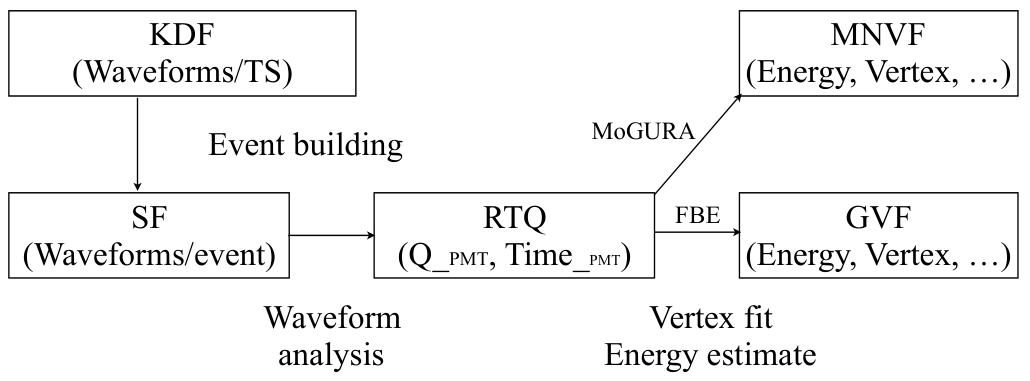
\includegraphics[scale=0.3]{dataflow.png}
	\caption{Data flow in KamLAND from raw waveforms to analysis variables such as energy, vertex, total hit PMTs, etc. \cite{ozaki_phd}}
	\label{fig:dataflow}
\end{figure}

GVF files contain the following information:
\begin{itemize}
	\item \textbf{run number}
	\item \textbf{event number}
	\item \textbf{TimeStamp} based on DAQ clock time (25 nsec for KamFEE, 20 nsec for MoGDAQ)
	\item \textbf{unixtime} is the number of seconds from January 1st in 1970 and used for some run vetos
	\item \textbf{trigger type} records which trigger was used
	\item \textbf{event vertex and badness} event vertices and a radius from detector center is saved, along with a vertex fit quality parameter called badness 
	\item \textbf{energy/energy17} visible energies given by the fitter, energy17 is the energy estimate only using 17-inch PMTs
	\item \textbf{TotalChargeID/17/OD} sum of all PMT charges of each PMT type
	\item \textbf{numhit/numhit17} the number of hit PMTs/17-inch PMTs in each event.
	\item \textbf{NsumMax} a maximum number of hit PMTs in a single DAQ cycle within each event, a "peak" nhit of the event
	\item \textbf{N200OD} Maximum number of simultaneous hit OD pmts within 200nsec windows
	\item \textbf{muon entrance and direction} muon fitter results are recorded.
\end{itemize}

Finally, MoGURA events are associated with muon events acquired in KamFEE DAQ (FBE) and stored in a Muon-Neutron Vector File (MNVF) to search for neutron capture events that occur shortly after muons.

\section{Event Reconstruction}
\subsection{Waveform Analysis}
Each digitized waveform has 128 samples with 1.5ns sample times; this corresponds to a waveform digitization window of 192 ns. The waveforms are processed and TQ reconstructed with the following procedure.
\begin{itemize}
	\item \textbf{Smoothing} Each waveform is smoothed via a running-average first derivate.
	\item \textbf{Baseline adjustment} The baseline of each PMT is collected at the beginning of each run. This baseline is subtracted from each waveform.
	\item \textbf{Peak finding} Peaks are found with running-averaged 1st, 2nd, and 3rd derivatives.
	\item \textbf{Leading-edge and Trailing-edge tag} A leading-edge is stamped as 10ns before the peak voltage. The trailing edge is stamped when the waveform returns to baseline. An example of this time-stamping is shown in Figure \ref{fig:waveform_analysis}
	\item \textbf{Waveform Sum calculation} The waveform is integrated from the leading-edge to the trailing-edge.
\end{itemize}

\begin{figure}[htb]
	\centering
	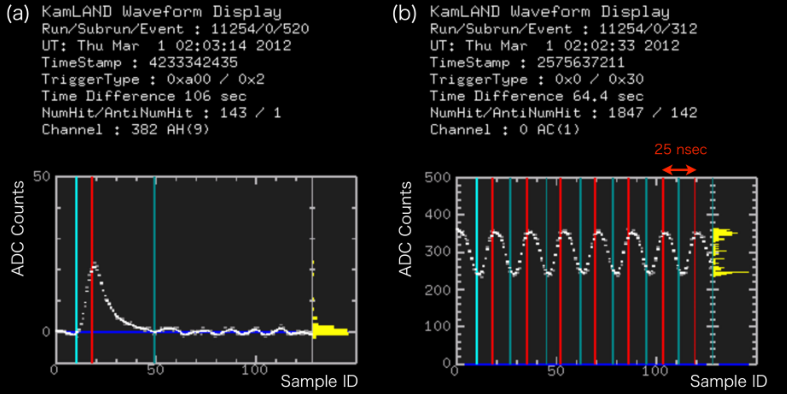
\includegraphics[scale=0.5]{waveform_analysis.png}
	\caption{An example of waveform analysis from thesis \cite{yoshida_phd}. (left) ADC counts of a real waveform after baseline subtraction. The left cyan line is the leading edge, the center red line is the peak position, and the right dark cyan line is a trailing-edge. (right) Clock calibration example on 25 nsec intervals.}
	\label{fig:waveform_analysis}
\end{figure}

When there are mulitple hits in one PMT waveform, the total charge of the hits and the earliest hit time is returned. This simplified information is used for the vertex and energy reconstruction. The multi-pe information is used for a double-pulse fit and a muon shower tag.

\subsection{PMT Corrections}
\subsection*{Low Gain Problem and HV Reductions}
Since ~2011, we observed that the gain of some of the 17-inch PMTs gradually decreased. As the gain of the PMTs fell, this compormises signal/background ratio and PMT waveform quality. It was also observed that the PMTs enter a low impedance state before the gain dropped. A HV current and voltage monitor allows for the real-time monitoring of this state. Usually a simple HV power cycle could recover normal PMT behavior. Since 2016, a auto HV power cycle mechanism was implemented to mitigate the low gain problem, but the root case is still unknown.

Each time the PMTs enter the low impedance state, the HV on that channel was reduced in 50-100 V increments. Over time, some of the channels had their HV reduced by 450 V. FIgure \ref{fig:lowgain_trend} shows the trend in low gain 17-inch PMTs.

\begin{figure}[htb]
	\centering
	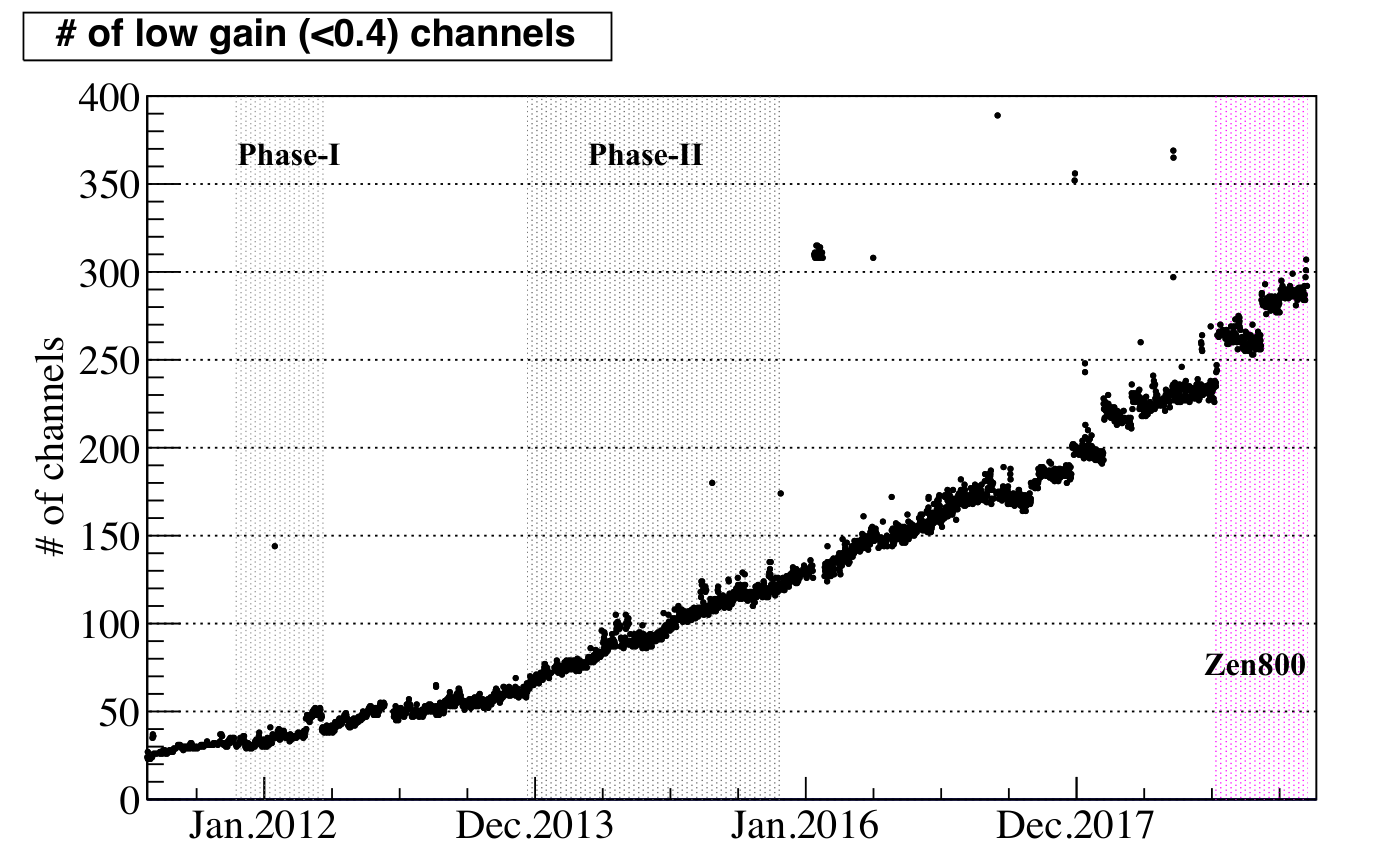
\includegraphics[scale=0.3]{lowgain_trend.png}
	\caption{The trend in the number of low gain 17-inch PMTs, before ZEN-800. The number of low gain channels increased gradually, while the sudden increases are from HV reductions performed since 2017 \cite{ozaki_phd}.}
	\label{fig:lowgain_trend}
\end{figure}

%/ TODO
Note about current low pmt gain analysis.

\subsection*{Bad Channel}
A channels is considered bad if the PMT meets one or more of the following criteria:
\begin{itemize}
	\item PMT pulses less than 0.6\% of the time over all events
	\item PMT pulses below 0.48\% for non-muon events
	\item PMT pulses less than 80\% of the time for high-energy muon events
	\item PMT is missing a waveform more than 10\% of the time
	\item Large discrepancy between the two ATWD hits
	\item High muon charge PMTs. A PMT may read much higher charge ($Q_{detected}$) than the average of its surrounding PMTs ($Q_{expected}$). A run is divided into 100 muon intervals, for each interval the criteria is defined as
	\[\frac{1}{N_{interval}}\sum_{i=1}^{N_{interval}}\left(\frac{1}{N_{muon}}\sum_{j=1}^{N_{muon}}\frac{(Q_{expected}-Q_{detected})^2}{Q_{expected}}\right)>1000\ p.e.\]
\end{itemize}
These bad channels are excluded from event reconstruction and physics analyses.

\subsection*{Dark Hit}
Thermal fluctuations can emit electrons off the photocathode leading to a PMT hit signal. These "dark hits" are an unavoidable hit-level background in PMT detectors, lowering the detector temperature reduces this effect. The dark hit rates are measured from run-to-run and are factored into our likelihood-maximizing reconstruction algorithms. The hit rate observed 50-100 ns before the PMT hittime rising edge is taken as the dark rate, Figure \ref{fig:darkrate} shows the PMT hittime distribution and the dark rate window.

\begin{figure}[htb]
	\centering
	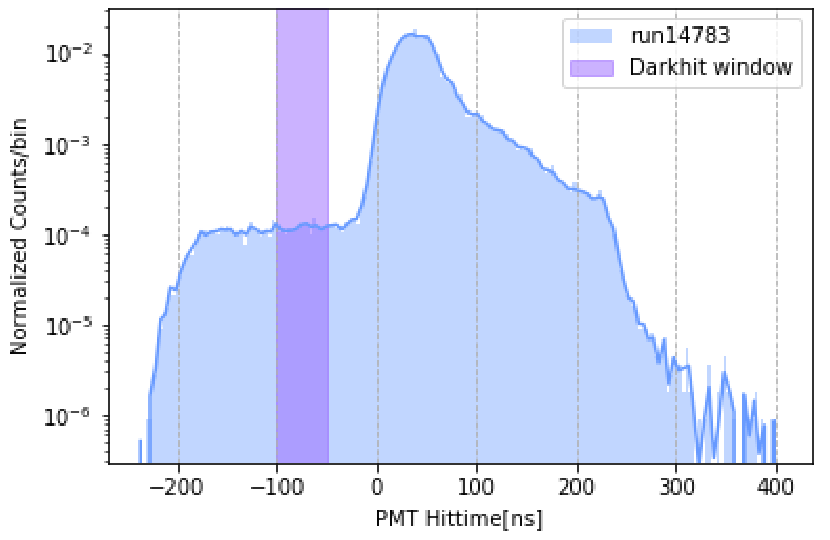
\includegraphics[scale=0.4]{darkrate.png}
	\caption{An example pmt hit time distribution from data run 14783, the 50-100 ns leading window is taken to measure the pmt dark hit rate. \cite{li_phd}.}
	\label{fig:darkrate}
\end{figure}

\subsection{Primary Vertex Fitter}
The primary vertex fitter provides a rough estimate of a scintillating event's location. This estimate serves as the input to a more thorough, but complex secondary fitter. The fit works by constructing a hit time residual distribution:
\begin{equation}
	T_{i}^{emit}=T_i-TOF_i = T_i - \frac{\left|R_i-r_{vertex}\right|}{c_eff}
	\label{eq:prim_vertex}
\end{equation}
Here $T_i$ is the hit time of the $i^{th}$ PMT, $TOF_i$ is the time it takes for a scintillation photon to traverse from the vertex position to the $i^{th}$ PMT position, $R_i$ is the PMT position, $r_{vertex}$ is the unknown vertex position to fit for, and $c_{eff}$ is the speed of light in the given medium. By fitting $T_i^{emit}$ to match the standard scintillation time profile, a primary $r_{vertex}$ is produced by the fitter.

\subsection{Secondary Fitter}
The secondary V2 fitter uses the $r_{vertex}$ given by the primary fitter to compute $T_0$ according to the equation \ref{eq:sec_v2}
\begin{equation}
	T_0 = \frac{\sum_i \left(T_i^{pmt}-TOF^{pmt}_i\right)\times Q_i}{\sum_iQ_i}- const.
	\label{eq:sec_v2}
\end{equation}
\begin{figure}[htb]
	\centering
	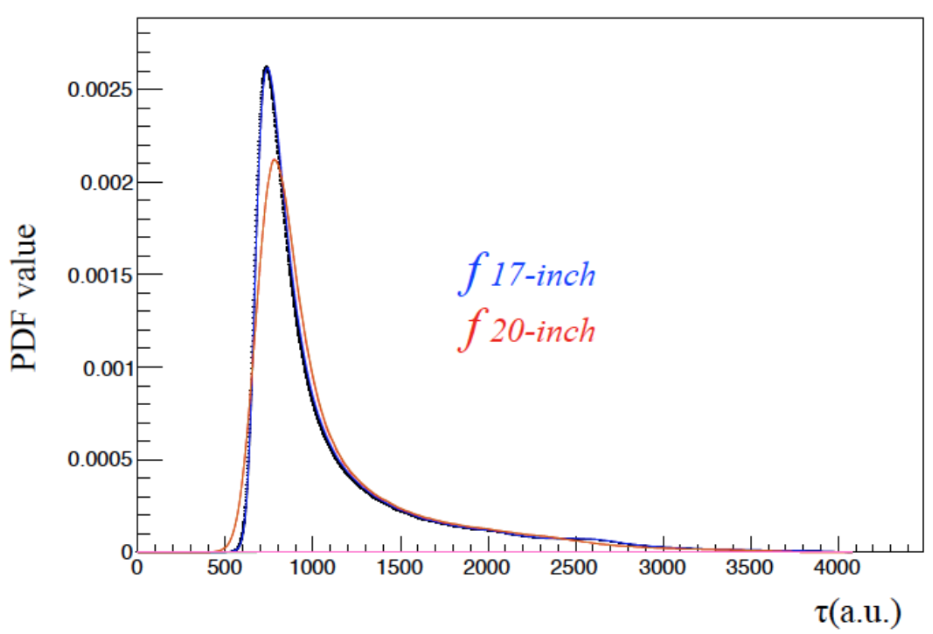
\includegraphics[scale=0.4]{pmt_dist.png}
	\caption{Probability density function of 17-inch and 20-inch PMT hit times calculated from calibration data. The plot is from \cite{ozaki_phd} and originally from a 2005 calibration dataset.}
	\label{fig:pmt_pdfs}
\end{figure}
This $T_0$ is the charge weighted sum of $T_emit$ from \ref{eq:prim_vertex}. This $T_0$ serves as the universal start point of an event. From this time, each pmt hit time is
\begin{equation}
	\tau(x,y,z,T_0) = T^{pomt}_i-TOF_i^{pmt}-T_0
\end{equation}
Finally, these time-of-flight corrected and centered hit time distributions are used to create probability distributions for the 17 and 20 inch PMTs respectively. These PDFs are shown in Figure \ref{fig:pmt_pdfs}. The likelihood function for an individual PMT is defined as:
\begin{equation}
	\phi_i =\frac{\mu\times f_i(\tau_i)+D_i}{\mu\times C_{17/20}+D_i}
\end{equation}
Here, $\mu$ is the pulse shape determination factor, $D_i$ is the dark hit rate for the $i^{th}$ PMT and $C_{17/20}$ is the normalization constant for the 17 or 20 inch PMTs. The overall log-likelihood is given by the $log(L)=\sum_ilog(\phi_i)$. The log-likelihood is maximized by the Newton-Raphson method, in which the $x,y,z,T_0$ are adjusted to the best-fit values, giving us the V2 reconstructed vertex.

\subsection{Energy Reconstruction}
\label{sec:energy_reco}
Likelihood maximization is also used to reconstruct the energy of an event. A likelihood PDF is constructed using the number of hits, charge, and hit timing.
\subsection*{$N_{hit}$ PDF}
The expectation of the number of photons hitting PMT i, $\mu_i$ is a function of the visible energy and dark charge.
\begin{equation}
	\mu_i = a_i(x,y,z)\times E_{vis} +d_i
\end{equation}
Here, $a_i(x,y,z)$ is a coefficient that converts the event energy to the number of photons which is calibrated with the neutron events. It is determined by the PMT position $x,y,z$. $d_i$ is the dark noise charge of PMT i, which is electronically measured. The probability that $\mu_i$ photons hit the $i$th PMT $j$ times, $k_{ij}$, is ideally expressed by the poisson distribution:
\begin{equation}
	k_{ij}=\frac{(\mu_i)^j}{j!}e^{-\mu}
\end{equation}

However, in KamLAND waveform analysis, the 1 p.e. detection efficiency is reduced by the 0.3 p.e. software charge threshold. This threshold is set to reduce the acceptance of dark noise but also decreases hit detection efficiency. As a result, the PMT hit probablity is reduced to:
\begin{equation}
	P_{hit}=1-v_ie^{-\mu_i}
\end{equation}

\subsection*{Hit Charge PDF}
A Gaussian distribution is assumed for the hit charge PDF of each PMT:
\begin{equation}
	f_{i,j(q_i)}=\frac{1}{\sqrt{2\pi j\sigma^2}}exp(-\frac{(q_i-j)^2}{2j\sigma^2})
\end{equation}
$q_i$ is the observed charge in p.e. units and $\sigma$ is  the charge resolution against 1 p.e. distribution.

\subsection*{Hit Time PDF}
PMT hit timing factors into energy reconstruction by helping to discriminate hits unrelated to the physical event. The hit timing model is created using source calibration data. 
\begin{equation}
	P_{time,i} = \frac{\psi(t_i)a_i E_{vis}+d_i}{\mu_i}
\end{equation}
The PDF is the sum of the signal hit distribution and the constant dark noise.
\subsection*{Energy Likelihood}
The likelihood function to be maximized is constructed as 
\begin{equation}
	L=\prod_{Not\ hit\ PMTs}P_{no-hit,i}\prod_{Hit\ PMTs}\left[P_{hit,i}\left(\sum_{j=1}^{100}f_{i,j}\right)P_{time, i}\right]
	\label{eq:energy_likelihood}
\end{equation}
The reconstructed energy is the one which maximizes this likelihood. The Newton-Raphson method is used to search for this energy. This process is implemented independently for the 17-inch PMTs and 20-inc PMTs, then the event energy is calculated with a weighting factor $\alpha$:
\begin{equation}
	E_{vis}=(1-\alpha)E_{17inch}+\alpha E_{20inch}
\end{equation}
The weighting factor $\alpha=0.3$ was determined to maximizing energy resolution.
\subsection*{Bad Channels in Energy Reconstruction}
The increase in the number of low gain PMTs has lead to worsening energy resolution over time, as these PMTs are excluded from the typical energy reconstruction described above. In particular, some of the low gain PMTs still detect photons, but proper gain calibration is not possible. A method for utilizing the information from operational low gain PMTs was developed, and the basic strategy is as follows:
\begin{enumerate}
	\item The change in gain causes the effect of the 0.3 p.e. threshold on hit probability to change. The no-hit probability was expanded as follows:
	\begin{equation}
		P^{\prime}_{no-hit, i} = \left(1+\epsilon_1\mu_i+\epsilon_2\frac{\mu_i^2}{2!}+\epsilon_3\frac{\mu_i^3}{3!}\right)e^{-\lambda\mu_i}
	\end{equation}
	This model was originally a simple expansion of $P_{no-hit}$, but in the end was adjusted phenomologically to better reproduce real data. This adjustment is why an additional $e^{-\lambda\mu}$ appears in the model.
	\item The parameters $\epsilon_1, epsilon_2, epsilon_3,$ and $\lambda$ are estimated with actual data. The events satisfying the following selections are collected and the no-hit probability is calcualted for each expected charge. The expected charge of the i-th PMT $\mu_i$ is estimated using the vertex and total charge of the events that meet the following conditions.
	\begin{itemize}
		\item $r<6m$
		\item Not muons or events within 2 ms after muons
		\item Events with more than 120 17-inch PMT hits
		\item PMT waveforms that contain only 1 peak
	\end{itemize}
	Figure \ref{fig:nohit_prob} shows the result of fitting this adjusted no-hit probability model. THe fitting is performed run-by-run and for each PMT independently.
	\item Use the updated no-hit probability pdf in the event energy reconstruction in Equation \ref{eq:energy_likelihood}.
\end{enumerate}
\begin{figure}[htb]
	\centering
	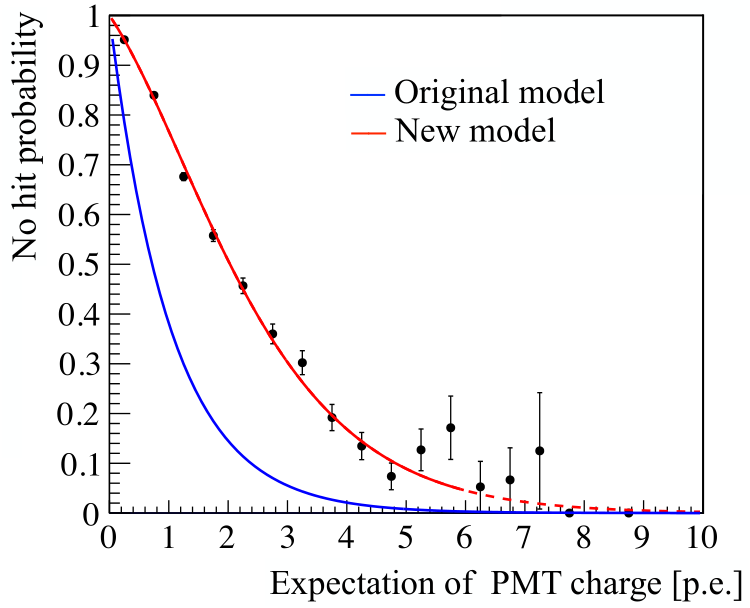
\includegraphics[scale=0.4]{no-hitprob.png}
	\caption{Fitting no hit probability to a low gain PMT against the expected charge $\mu$. The original model is shown with the blue line while the red line is the new model which agrees better with low-gain PMT data.}
	\label{fig:nohit_prob}
\end{figure}

Making use of the low-gain PMTs can improve energy resolution by up to 3\% \cite{karino_master}. Further analysis in this work uses energy reconstructed from the combination of normal and low-gain PMTs.

\subsection{Muon Reconstruction}
The selection and understanding of muon and muon-correlated neutrons are essential to multiple background rejections. This section, describes the special selection criteria and reconstruction methods used for muons and neutrons.
\subsection*{Muon Selectrion Criteria}
The muon event selection criteria are as follows:
\begin{itemize}
	\item Total charge of 17inch PMTs, $Q_{17}\geq 10000$ p.e.
	\item $Q_{17geq}$ 500 p.e. and the number of hit OD PMTS $\geq 9$.
\end{itemize}
The former criteria selects muons which go through the scintillator volumes of the detector. A total charge of 10,000 p.e. roughly corresponds to an event energy of 30 MeV, which exceeds the energy range of most physical analyses in KamLAND-ZEN. The second selection is for muons that only deposit energy in the outer buffer oil (clipping muons). Muons passing through the buffer oil volumes do not scintillate, as such the 500 p.e. threshold in Chrenkov radiation roughly corresponds to about 40 MeV of energy deposition.
\subsection*{Cosmic Ray Muon Reconstruction}
Cosmic ray muon events form tracks as opposed to the point-like events caused by single decay events. The process is shown diagramattically in Figure \ref{fig:muon_reco}
\begin{enumerate}
	\item The ID PMT which detects the earliest light is identified. If the charge of this hit is low or isolated in time from the many other hits in the event, it is classed as a dark hit and ignored. A line is drawn from the earliest hit muon PMT and the center of the KamLAND detector. The intersection of this line and the outer balloon is marked as the temporary entrance point.
	\item The PMT whose charge is the largest is identified. The brightest hit PMT should be hit later than the earliest PMT and the neighbors of the earliest PMTs. A line is drawn from the brightest hit PMT and the center of the KamLAND detector. The intersection of this line and the outer balloon is marked as the temporary exit.
	\item The temporary track is defined as the line connecting the temporary entrance and exit. The temporary track is finally corrected by checking the correlation between the track length and the total charge.
	\item The reconstruction quality is evaluated by checking the following:
	\begin{itemize}
		\item Whether the earliest and the brightest PMTs can be identified
		\item Whether the mean hit time of PMTs around the entrance is earlier than the around the exit.
	\end{itemize}
	A "badness" parameter value is assigned to the reconstruction according to this evaluation. With this evaluation, around 15\% of muon candidates are regarded as badly reconstructed though they can still be used in muon-neutron pairing. Bad muon reconstruction is caused by ringing in the PMT signals, muon bundles, and stopped muons.
\end{enumerate}
The light yields in the muon events are estimated in \cite{karino_master}:
\begin{equation}
	\langle dQ_C/dX\rangle =28\pm 5\textbf{p.e./cm (Cherenkov muons)}
\end{equation}
\begin{equation}
	\langle dQ_S/dX\rangle =338\pm 12\textbf{p.e./cm (Scintillation muons)}
\end{equation}
\subsection{MoGURA Neutron Reconstruction}
Neutrons that are produced during cosmic ray spallation are best detected with the MoGURA DAQ due to the FBE's inability to handle the high after-pulse rate. After pulsing is also present in MoGURA and need to be rejected. An effective number of hits $N_s$ was introduced. The neutron reconstruction procedures is as follows:
\begin{enumerate}
	\item A 200ns wide time window is opened. The vertex is reconstructed using LT Vertex using the hit information contained in this window.
	\item The times of flight to each PMT is calculated assuming the reconstructed vertex. Then the ToF subtracted hit timing distribution is obtained.
	\item The obtained residual hit time distribution includes neutron capture 2.2 MeV gamma scintillation light and fake signals from after-pulses. To calculate the effective number of hits, $N_{in}$ and $N_{out}$, the number of hits in a 30ns wide "ontime" window and a 170ns wide "offtime" window respectively are counted. $N_s$ is then calculated as
	\begin{equation}
		N_s=N_{in}-N_{out}\times\frac{30 nsec}{170 nsec}
	\end{equation}
	\item The ontime window is shifted by 20ns, the clock time of MoGDAQ, and step 3 is repeated.
	\item The 200ns time window is shifted and steps 1-4 are repeated. the 200ns window and 30ns ontime window that maximizes $N_s$ is found. The vertex given by the $N_s$ maximizing time windows is taken as the reconstructed neutron capture event vertex.
\end{enumerate}
\begin{figure}[htb]
	\centering
	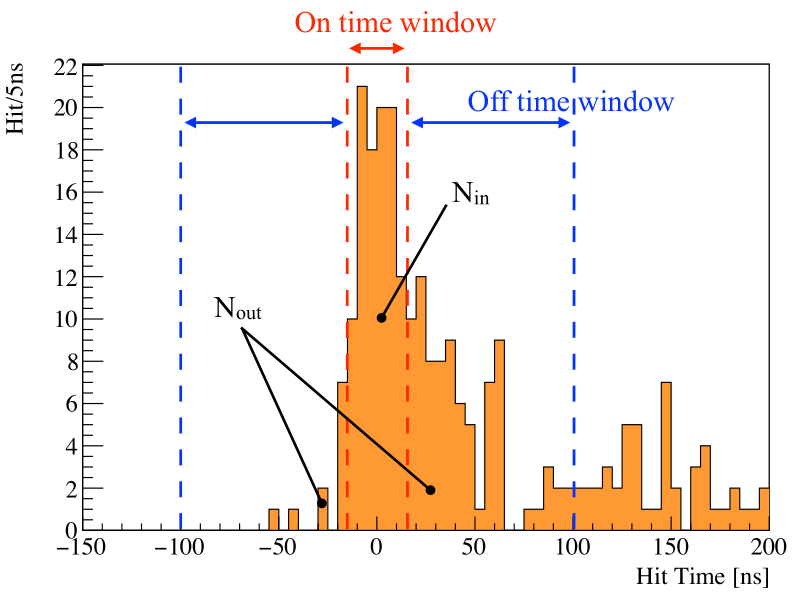
\includegraphics[scale=0.4]{neutron_reco.png}
	\caption{A neutron capture events hit times showing the contribution of fake after pulses and the time windows used to calculate $N_s$}
	\label{fig:neutron_reco}
\end{figure}
\subsection{Muon Neutron Correlation}
The neutron selection process outlined above contains many noise events, thus the sample is only used in background discrimination when coincident with muons. In particular, MoGURA data neutrons are used to improve the rejection of xenon spallation products. The procedure for selecting muon-neutron pairs is:
\begin{enumerate}
	\item Check the end unixtime of the previous KamDAQ run and the start unixtime of the current KamDAQ run.
	\item Collect the MoGURA runs that collected data during this gap. Muon events collected by MoGURA are used in the gaps between KamDAQ runs, during KamDAQ runs muons collected with FBE data are used.
	\item The delayed coincidence analysis is done to select neutron candidate events in a short time period after muons. The first cuts applied are on $dT>2500\mu $ and $N_{s}=N_{in}-N_{out}<100$, these events are first removed. The subsequent MoGURA neutron selection criteria are outlined below.  
\end{enumerate}

The neutron selection in MoGURA is outlined in Figure \ref{fig:neutron_selection}. Two quantities are used, $dT$, the time delay between the neutron event and the previous muon, and $N_s$. From the 2D distribution, one sees that the event rate is higher in the short dT region due to noise and after-pulses. The $N_s$ values also tend to be small due to signal loss caused by baseline overshoot in the PMTs. The following criteria were chosen to select MoGURA neutrons:
\begin{itemize}
	\item $N_{total}=N_{in}+N_{out}>150$ (Number of hit requirement)
	\item $N_s>50 \wedge 10<dT<1200\mu s $ (reject after-pulses and accidental events)
	\item $!((N_s<dT(\mu s)+70\wedge 10<dT<20 \mu s )||N_s<-0.8\times dT(\mu s)+106\wedge20<dT<70\mu s)$
\end{itemize}
Figure \ref{fig:neutron_dT} shows the dT distribution of the MoGURA neutrons collected with the above criteria. The histogram is fitted to an exponential between 500 and 1000 $\mu s$, and the fitted function is extrapolated to the rest of the data range. The inefficiency of the neutron tag in the shorter dT period can be seen as the distribution turns off at low dT.

\begin{figure}[htb]
    \begin{minipage}{0.5\textwidth}
        \centering
        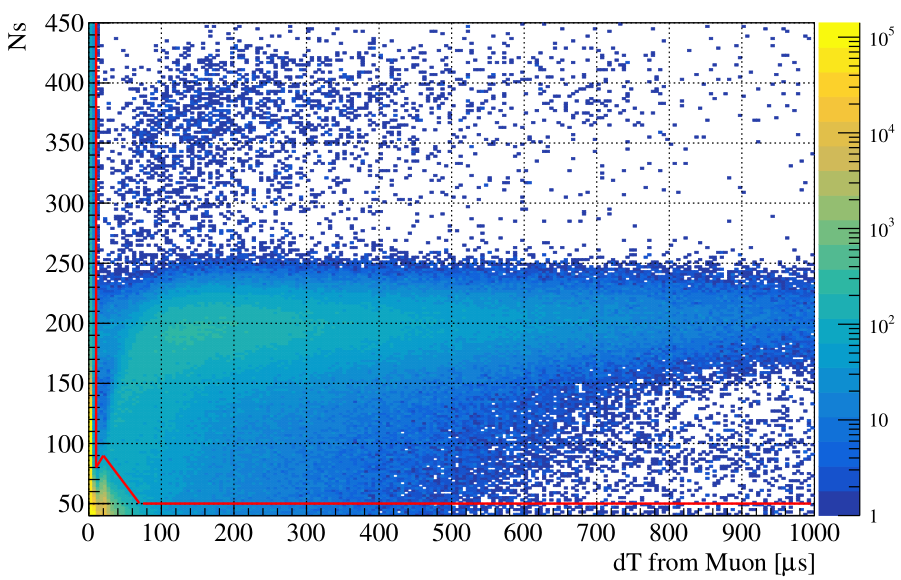
\includegraphics[scale=0.3]{mog_neutron.png}
        \caption{distribution showing the $dT$ dependence of $N_s$. The events above the red line are selected as MoGURA neutrons and used for background rejection \cite{takeuchi_phd}}
        \label{fig:neutron_selection}
    \end{minipage}
    \hfill
    \begin{minipage}{0.5\textwidth}
        \centering
        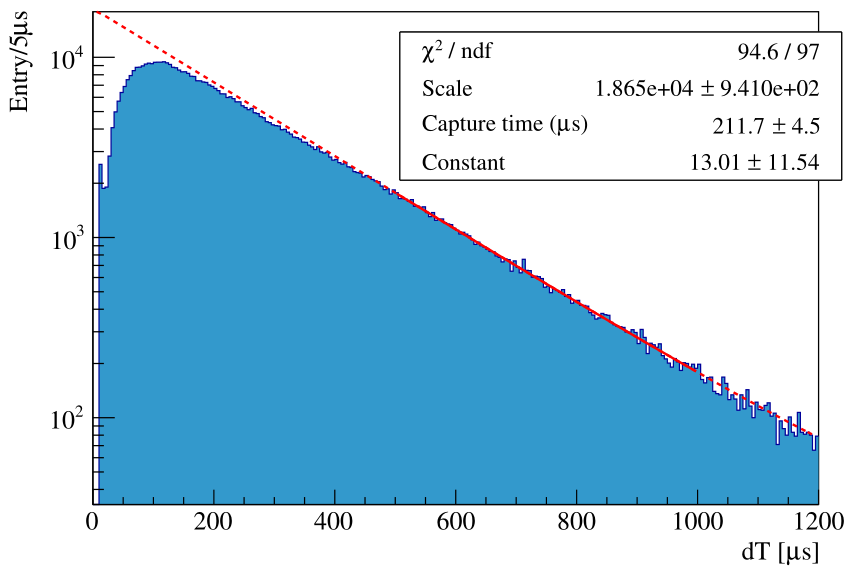
\includegraphics[scale=0.3]{mog_neutron_dt.png}
        \caption{The $dT$ distribution of selected MoGURA neutrons. The fit to an exponential is performed between 500 and 1000 $\mu s$. \cite{takeuchi_phd}}
        \label{fig:neutron_dT}
    \end{minipage}
\end{figure}

\section{Event Selection}
Candidate \0nbb events must pass several event selections. The selections are separated into non-physical events and background cuts. In this section, we first describe the event selections used in this analysis. Then, the impact of these selections on signal inefficiency are discussed.

\subsection{Unphysical and Bad Quality Event Rejection}
\label{sec:badqualityevents}
Much of the data saved in the KamLAND DAQ systems include "unphysical" events. Furthermore, much of the events associated with real physical processes are of poor quality. This section, describes the criteria by which unphysical events and poor quality events are selected.
\begin{enumerate}
	\item Flasher PMT \\
	PMTs, can occasionally emit light into the detector. These occurances are called PMT flashers. There are multiple potential causes for a PMT to flash, such as the discharge of the dynodes and light emission from the epoxy around the breeder circuit. Figure \ref{fig:flasher} shows the typical event display of a flasher event. Such events have a distint signature, as the PMT that flashes will have exceptionally high charge and cause a huge deposition of charge in the nearest PMTs as well. The PMT flasher selection criteria are as follows:
	\begin{itemize}
		\item Total charge of ID PMTs $ > 2500$ p.e.
		\item Maximum ID PMT charge/Total ID PMT Charge $ >60\%$
		\item Average charge of the neighboring PMTs $ > 20$ p.e.
	\end{itemize}
	\begin{figure}[htb!]
		\centering
        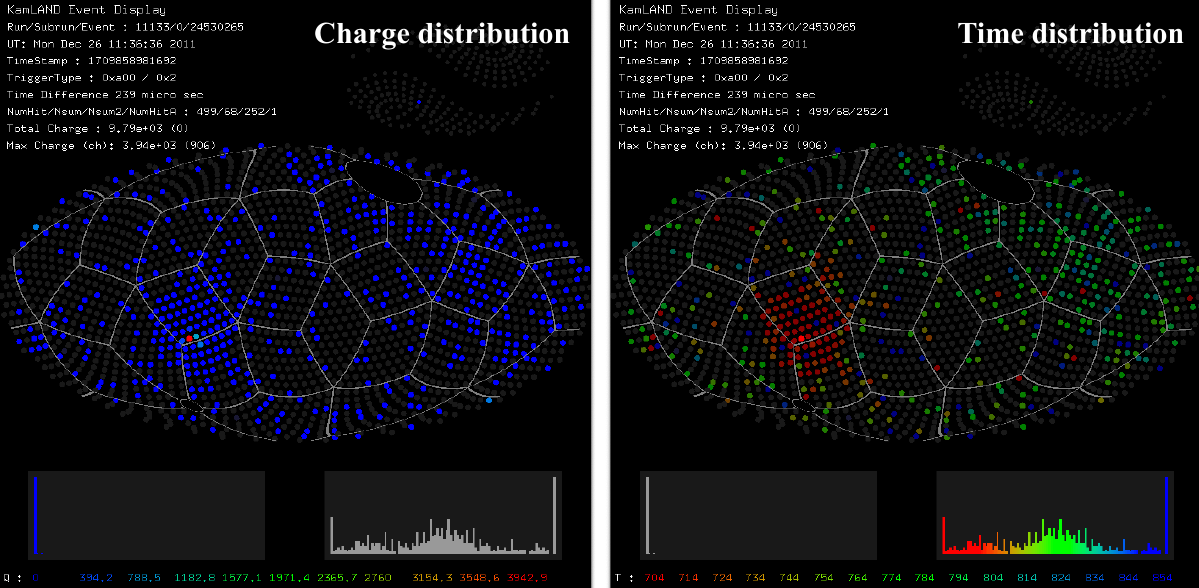
\includegraphics[scale=0.45]{flasher.png}
        \caption{Event display of a flasher event. The left shows the charge distribution. One PMT has an exceptionally large charge. Right shows the time distribution. It is relatively flat since the source is not scintillator. The hit timing of the flasher PMTs and its neighbors are very early.}
        \label{fig:flasher}
	\end{figure}
	\item Post muon events \\
	Cosmic ray muons deposit a large amount of energy into the detector. As a result, the detecotr behavior is unstable for a period afterwards. In particular, the detector suffers from a high fake event rate due to after-pulsing and the shift of baseline from overshoot. This instability causes not only a large amount of unphyiscal events, but also degrade the reconstructibility of real physical events. Thus, all events in the immediate 2 msec after cosmic ray muons are not uesd for the excited state analysis. Though, these events may be used for other analyses such as spallation background estimation.
	\item Missing waveform events \\
	High rate after-pulsing from cosmic ray muons can also cause the ATWD to be busy and the DAQ system to get stuck. When the DAQ electronics are in this state, event waveforms cannot be recorded. These are referred to as "missing waveform" events. In these situations, the number of hit 17-inch PMTs within 125 ns after a trigger issue is recorded as "NsumMax". In properly recorded events, NsumMax should be proportional to the total number of 17inch PMT hits (Nhit17). So the missing waveform events are identified by the ratio between NsumMax and Nhit17; the distributions of these two quantities are shown in Figure \ref{fig:missing_waveform}. Events tagged by this selection are removed from the excited state physics analysis. The exact selection criteria are as follows:
	\begin{itemize}
		\item Nhit17 $<$ NsumMax $\times 0.99-25$
		\item $dT$ after muon events $< 2$ msec (if NsumMax<1200)
		\item $dT$ after muon events $< 2$ sec (if NsumMax>1200)
	\end{itemize}
	\begin{figure}[htb]
		\centering
        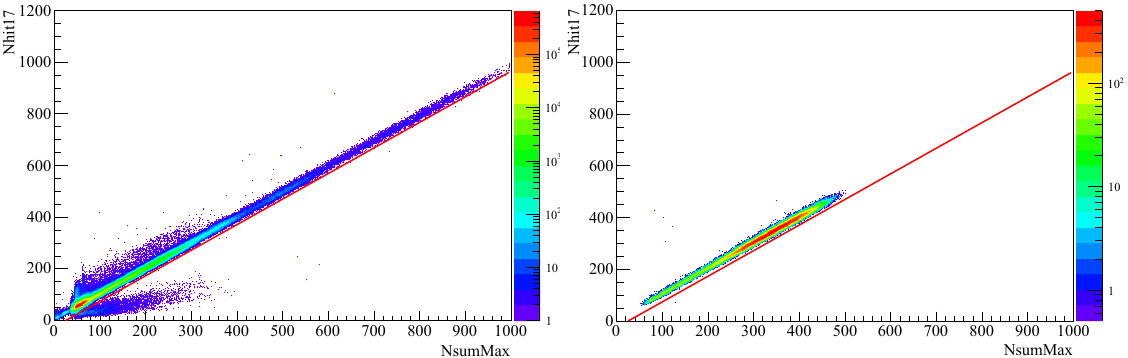
\includegraphics[scale=0.45]{missing_waveform.png}
        \caption{Nhit17 vs NHitSumMax distributions for all physics events (left) and Bi214-tagged events (right). The missing waveform cut inefficiency can be calculate from the Bi214-tagged events to be $< 0.01\%$}.
        \label{fig:missing_waveform}
	\end{figure}
	\item Post PPS trigger event \\
	The PPS trigger is a forced trigger issued once a second used for constant diagnostic monitoring of the detector. However, the PPS trigger has been found to cause an increase in electronics noise and DAQ trigger rate. Thus events 100 $\mu sec$ from the last PPS trigger are removed from the analysis.
	\item Badly reconstructed events \\
	The fit quality of an event's vertex reconstruction is the event's "Badness". The quantity is calculated using nine parameters that describe the deviation of an event's PMT hit and charge distribution from the expectation. A detailed explanation of the Badness calculation can be found in section 3.8.3 of \cite{}. These poorly reconstructed events mostly consist of, noise events and pileup. The events with large Badness are removed from the analysis by the following energy-dependent threshold:
	\begin{equation}
		Badness < 25.0\times exp(-4.5\times E_{vis} [MeV]) + 3.1
	\end{equation}
	Figure \ref{fig:badness} shows the Badness distribution of all physical events and the Badness of $^{214}$Bi events selected by the delayed coincidence method.
	\begin{figure}[htb]
		\centering
        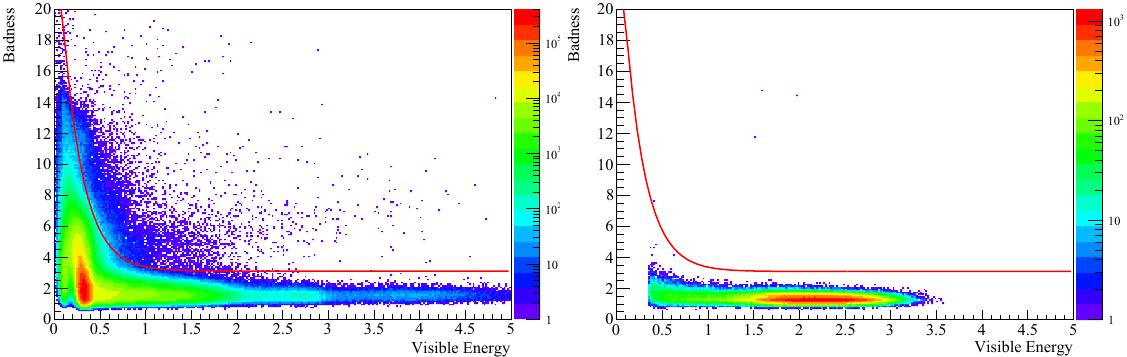
\includegraphics[scale=0.45]{badness.png}
        \caption{The badness distributions of all physics events (left) and Bi214-tagged events (right)}
        \label{fig:badness}
	\end{figure}
\end{enumerate}

\section{Background Rejection}
\subsection{Uranium/Thorium}
$^{214}$Bi and $^{212}$Bi are radioactive nuclei produced in the uranium and thorium decay series, respectively. They are among the dominant backgrounds in KamLAND-ZEN. These isotopes are introduced to the detector primarily by Uranium/Thorium contamination in the LS itself or on the surface of the inner balloon. There were also some $^{222}$Rn introduced when the XeLS was filled, this decayed with a half-life of 3.8 days, as such the $^{222}$Rn-related $^{214}$Bi decayed away in the early stages of KamLAND-ZEN 800. This time-dependence of the Radon background is accounted for in the physics analysis.
These Bismuth-decays are tagged in two ways: Delayed-coincidence veto and Double-pulse fitting.
\subsection*{Delayed Coincidence Veto}
Both $^{214}$Bi and $^{212}$Bi decays are quickly followed by the decays of $^{214}$Po/$^{212}$Po:

\begin{equation}
\begin{aligned}
&^{214}\mathrm{Bi}
\ \xrightarrow[\substack{19.9\,\mathrm{min},\ 99.98\%}]{\beta^-,\ Q=3.27\,\mathrm{MeV}}
\ ^{214}\mathrm{Po}
\ \xrightarrow[\substack{164.3\,\mu\mathrm{s}}]{\alpha,\ Q=7.83\,\mathrm{MeV}}
\ ^{210}\mathrm{Pb}
\end{aligned}
\end{equation}

\begin{equation}
\begin{aligned}
&^{212}\mathrm{Bi}
\ \xrightarrow[\substack{60.55\,\mathrm{min},\ 99.98\%}]{\beta^-,\ Q=2.25\,\mathrm{MeV}}
\ ^{212}\mathrm{Po}
\ \xrightarrow[\substack{0.299\,\mu\mathrm{s}}]{\alpha,\ Q=8.95\,\mathrm{MeV}}
\ ^{208}\mathrm{Pb}
\end{aligned}
\end{equation}
These decays are correlated in space and time in KamLAND, they can be vetoed by searching for this correlation. The criteria of the Bi-Po delayed coincidence analysis used in the KamLAND-ZEN analysis is as follows:
\begin{itemize}
	\item delayed energy : $0.2 < E_d < 1.3$ MeV
	\item distance between prompt and delayed vertices : $dR<170$ cm
	\item timing delay between prompt and delayed vertices : $dT<1.9$msec
\end{itemize}

Figure \ref{fig:BiPo214} shows the delayed-coincidence veto parameter distributions used in the $^{214}$Bi selection. Coincident pairs within 10 $\mu sec$ are excluded and set aside for the $^{212}$Bi selection, as $^{212}$Po has a much shorter half-life. The delayed energy deposition distribution, two peaks are found. THe lower energy peak corresponds to polonium decays in which some energy is deposited not in the liquid scintillator but in the mini-balloon nylon film.
\begin{figure}[htb]
	\centering
	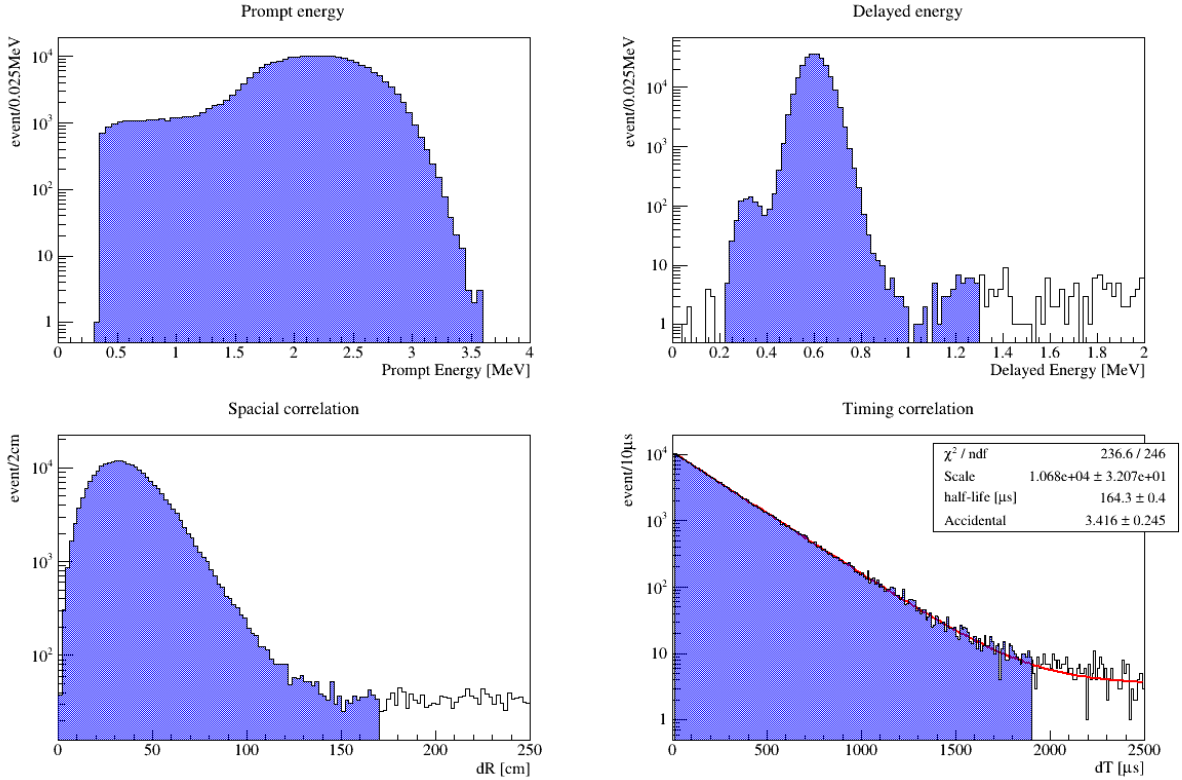
\includegraphics[scale=0.45]{bi214.png}
	\caption{The delayed coincidence selection parameters for $^{214}$Bi. The distributions of prompt energy, delayed energy, displacement, and delay time are shown. The blue shaded regions indicate the tagged events. Events with $dT<10\mu sec$ are set aside for $^{212}$Bi-Po selection.}
	\label{fig:BiPo214}
\end{figure}
Figure \ref{fig:BiPo212} shows the delayed-coincidence veto parameter distributions used in the $^{212}$Bi selection. For this selection, the timing selection is $dT<10\mu sec$. The veto efficiency of $^{214}$Bi-Po decays in the XeLS is $99.89\pm0.03\%$. The veto efficiency of $^{214}$Bi-Po decays in the balloon film is $48.9\pm9\%$. The lower veto efficiency is due to alpha decays depositing their energy in the film not the liquid scintillator. For $^{212}$Po decays that occur immediately after the initial $^{212}$Bi decay, they can be tagged by the double pulse fitter, which the next section describes.
\begin{figure}[htb]
	\centering
	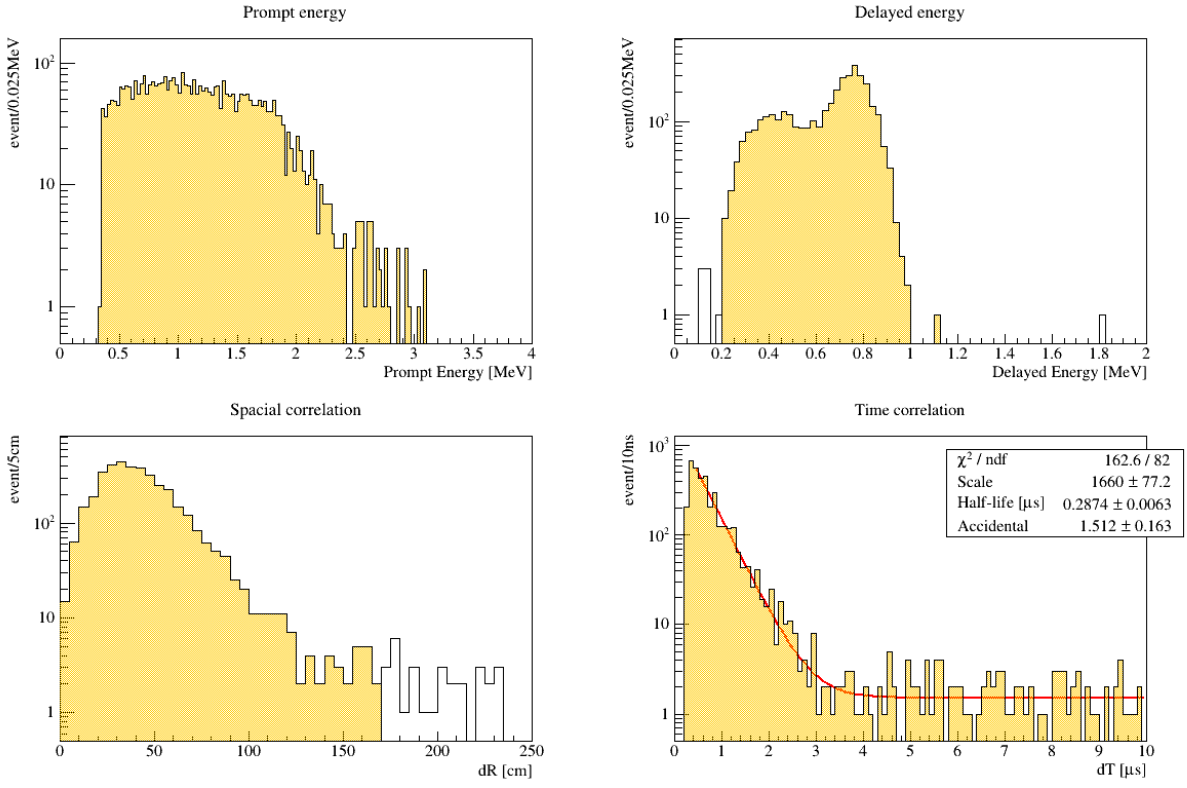
\includegraphics[scale=0.45]{bi212.png}
	\caption{The delayed coincidence selection parameters for $^{212}$Bi. The distributions of prompt energy, delayed energy, displacement, and delay time are shown. The yellow shaded regions indicate the tagged events. Only events with $dT<10\mu sec$ are used for this selection.}
	\label{fig:BiPo212}
\end{figure}
\subsection*{Pileup Events}
\label{sec:dpfit}
When the delay time, $dT$, between prompt and delayed events are small enough, Bi-Po sequential events can be stored as a single event in KamLAND's data acquisition window. In these cases, the delayed coincidence selection of two related events does not work. Such events are referred to as pile-up events. Since these pileup events contain the kinetic energy of the initial beta decay and the subsequent alpha decay, the combined deposited energy reaches beyond the \0nbb ROI and becomes an important background to reduce. The energy spectrum of these $^{212}$Bi-Po pile-up events are shown in Figure \ref{fig:BiPo_energy}.

A double pulse fit method has been developed to tag these pile-up events. The method simply searches for events with a hit-timing distribution indicative of two distinct energy depositions, or hit time peaks. The hit time distribution of an event is fitted with 2 reference waveforms by the following procedure:
\begin{enumerate}
	\item Construct a reference time profile.
	A reference waveform is made from the hit time profile of \2nbb-decay candidates. The events are selected with $1.4 < E_{vis}<1.6$ MeV and $radius < 157$ cm after \0nbb background vetoes. 
	\item Construct the hit timing profile of \0nbb decay candidates.
	The hit timing profile of the candidate events (events to be analyzed) are constructed. In the typical analyses and reconstructions, the time of the first hit on a PMT in an event is used. For this procedure, all hit times and hit charges (multi-hit) information is used to effectively separate the two peaks. 
	\item Fit the event's hit time profile
	The hit time profile is fitted by the reference waveform. The fit includes 4 parameters; $E_p$ (prompt signal energy), $T_p$ (prompt signal timing), $E_d$ (delayed signal energy), $\Delta T$ (time delay between prompt and delayed signals). Then a maximum likelihood optimization is performed. $\chi^2$ for the fit is defined as:
	\begin{equation}
		\chi^2 = 
		\begin{cases}
		2\sum_i \left\{ -(x_i-f_i) + x_i \log \frac{x_i}{f_i} \right\} & (n_i > 0) \\
		2\sum_i \left\{ -(x_i-f_i) \right\} & (n_i = 0)
		\end{cases}
		\hspace{2cm} (5.27)
	\end{equation}
	where $i, x_i$, and $f_i$ denote the $i$-th bin, the number of hit PMTs in the $i$-th bin and the expectation of hte number of hits in the $i$-th bin, respectively. The time bins are 1 ns wide. $f_i$ can be calculated as the sum of a dark rate $D$ and the reference waveform $R(i)$ as:
	\begin{equation}
		F_i = |E_p|R(i-T_p)+|E_d|R(i-T_p-\Delta T) + D
	\end{equation}
	Here, the dark rate is a simple global dark rate taken from all the PMTs in the off-time period. The $chi^2$ minimization is performed with MINUIT in the ROOT analysis framework. For all the $(T_p, \Delta T)$ pairs, $E_p$ and $E_d$ are floated, and the optimal four parameters are found.
	\item Correct the reconstructed energies
	$E_p$ and $E_d$ are used in the double-pulse fit to scale the reference waveform but they are not accurate individual pulse energy reconstructions. The energy reconstruction described in section \ref{sec:energy_reco} is more accurate. This "official" energy reconstruction is incorporated into the individual pulse energies by:
	\begin{equation}
		E_{p^\prime}=E_{vis}\times\frac{E_p}{E_p+E_d}
	\end{equation}
	\begin{equation}
		E_{d^\prime}=E_{vis}\times\frac{E_d}{E_p+E_d}
	\end{equation}
	Thus, the double-pulse fit provides the fraction of the total event energy, $E_{vis}$, to assign to the prompt and delayed signals.
	\item Candidate selection
	Finally, the pile-up tagged events are selected from the candidate events based on their $\Delta T$ and $E_{d^\prime}$. The selection criteria are determined using MC simulated events while limiting the \0nbb inefficiency to about 0.1\%. Figure \ref{fig:pileup_selection} shows the selection criteria over the MC distributions. The remaining $^{212}$Bi-Po events that pass pile-up are estimated to be $2.3\pm0.5\%$.
\end{enumerate}
\begin{figure}[htb]
	\centering
	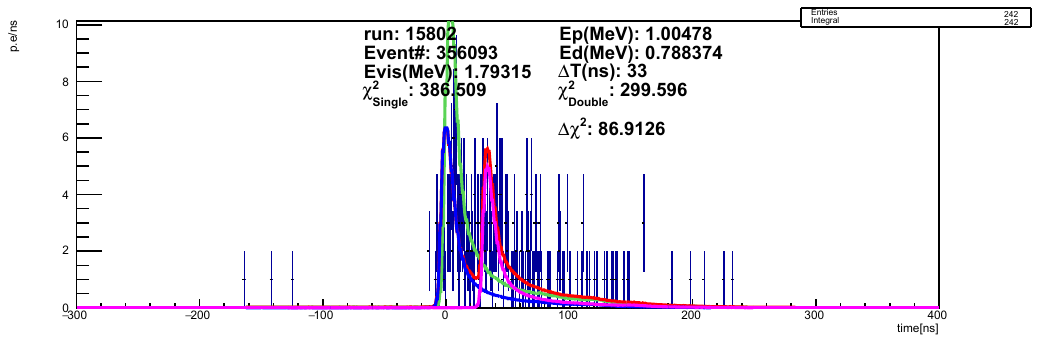
\includegraphics[scale=0.5]{highE_example_doublepulse.png}
	\caption{An example double pulse fit result, The green line shows the fit result using a single reference waveform. The red line shows the double-pulse fit. The blue and magenta curves show the prompt and delayed pulses respectively.}
	\label{fig:dpfit}
\end{figure}
\begin{figure}[htb]
	\centering
	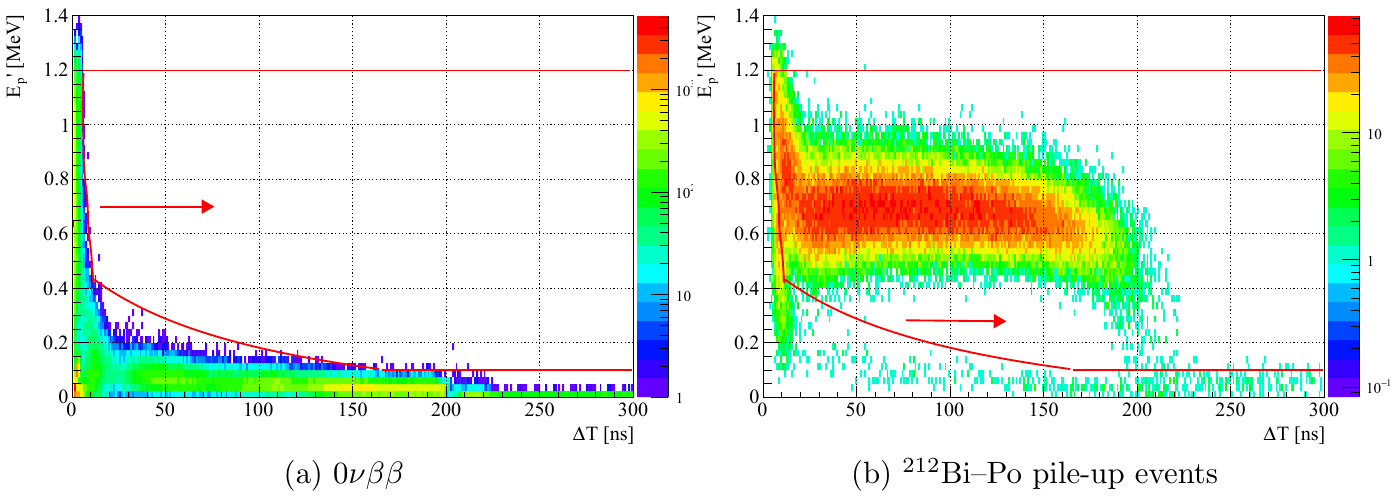
\includegraphics[scale=0.35]{dp_selection.png}
	\caption{The selection criteria over $E_d$ and $\Delta T$ used to tag pileup events. The distributions are of MC \0nbb (left) and $^{212}$Bi-Po (right). The regions enclosed by the red lines are vetoed as pileup events.}
	\label{fig:pileup_selection}
\end{figure}
An example double-pulse fit is shown in Figure \ref{fig:dpfit}. This double-pulse fitting technique has also been used to identify other pile-up like backgrounds. For example, some of the $\beta^+$-decay backgrounds can be rejected by this method. The ortho-positronium decay mode of $\beta^+$-decays has a lifetime of about 3 ns in the liquid scintillator, which produces a pileup-like signal.

\subsection{Antineutrinos}
The original physics objective of the KamLAND experiment was to observe electon anti-neutrinos produced in nuclear reactors, among other sources. The signature of anti-neutrinos in KamLAND and KamLAND-ZEN is inverse beta decay (IBD):
\begin{equation}
	\bar{\nu_e}+p\rightarrow e^+ + n
\end{equation}
IBD produces a neutron and a positron. The positron annihilates with an electron to produce gamma rays, 2 511 keV gammas. The neutron scatters in the detector until being captured by protons with an average capture time of $\tau=207\mu s$. This two-stage signal is ideal for tagging with the delayed coincidence method.

In the anti-neutrino analysis, IBD events were originally selected by a likelihood ratio selection; but in KLZ, a simple box cut analysis is applied. The IBD selection criteria are:
\begin{itemize}
	\item delayed energy : $E_d>1.5 MeV$
	\item distance between prompt and delayed vertices : $dR<200cm$
	\item timing correlation between prompt and delayed vertices : $dT < 1.0msec$
\end{itemize}
In the wake of the 2011 Tohoku earthquake and reactor meltdown, the Japanese nuclear power plants were turned off and the rate of anti-neutrino events are less than 0.2 event/day within $r<550$ cm. The efficiency of the IBD box cuts are 99.14\%. Thus, the remaining potential IBD background to the KLZ analyses are negligible.
\subsection{Short-lived Spallation Products}
High energy cosmic ray muons can break apart nuclei in the detector material into lighter nuclei and produce secondary particles. The spallation products of $^{12}$C are one of the dominant backgrounds in the $2n\beta\beta^*$ search. Multiple tagging methods have been developedfor identifying so-called short-lived spallation products.
\subsection*{$^{12}$B Veto}
The $^{12}$B $\beta$-decay has a large contribution to the background in the \0nbb ROI. The rate of muons is $\approxeq 3$ Hz in the KamLAND detector thus $^{12}$B can be removed with a veto after muons. In this analysis, a 150 msec window, corresponding to 5 times the livetime of $^{12}$B, is vetoed and counted as detector deadtime.

\subsection*{MoGURA Neutron Veto}
Neutrons are also ejected during the muon spallation process. These neutrons are correlated with the spallation products. The MoGURA DAQ system is used to observe neutron captures that occur shortly after cosmic-ray muons. The correlation with these MoGURA neutrons can be used to tag other short-lived spallation products, mainly $^{10}$C, $^{6}$He, and $^{8}$Li. The selection of the MoGURA neutron veto is as follows:
\begin{itemize}
	\item distance between candidate decay and spallation neutron : $dR<160$ cm
	\item timing correlation : $dT < $ 180 sec ( about 5 times the lifetime of $^{10}$C)
\end{itemize}

\subsection*{$^{137}$Xe Veto}
Neutrons capturing onto $^{136}$Xe nuclei form $^{137}$Xe. The Q-value of $^{137}$Xe $\beta^-$-decay is 4.2 MeV with a half-life of 3.82 minutes. This decay can be tagged by the triple coincidence of a muon, the neutron capture, and the beta decay itself. The selection criteria is as follows:
\begin{itemize}
	\item distance between candidate decay and spallation neutron : $dR<160$ cm
	\item timing correlation : $dT < $ 1,620 sec
\end{itemize}

Since the neutron capture gamma on $^{137}$Xe has a gamma energy about 4 MeV, higher than captures on protons, the neutron selection criteria is adjusted slightly. The $^{137}$Xe neutrons are required to have $N_s$ values above 240. A schematic of spallation veto of Carbon and Xenon is shown in Figure \ref{fig:spall_veto}.
\begin{figure}[htb]
	\centering
	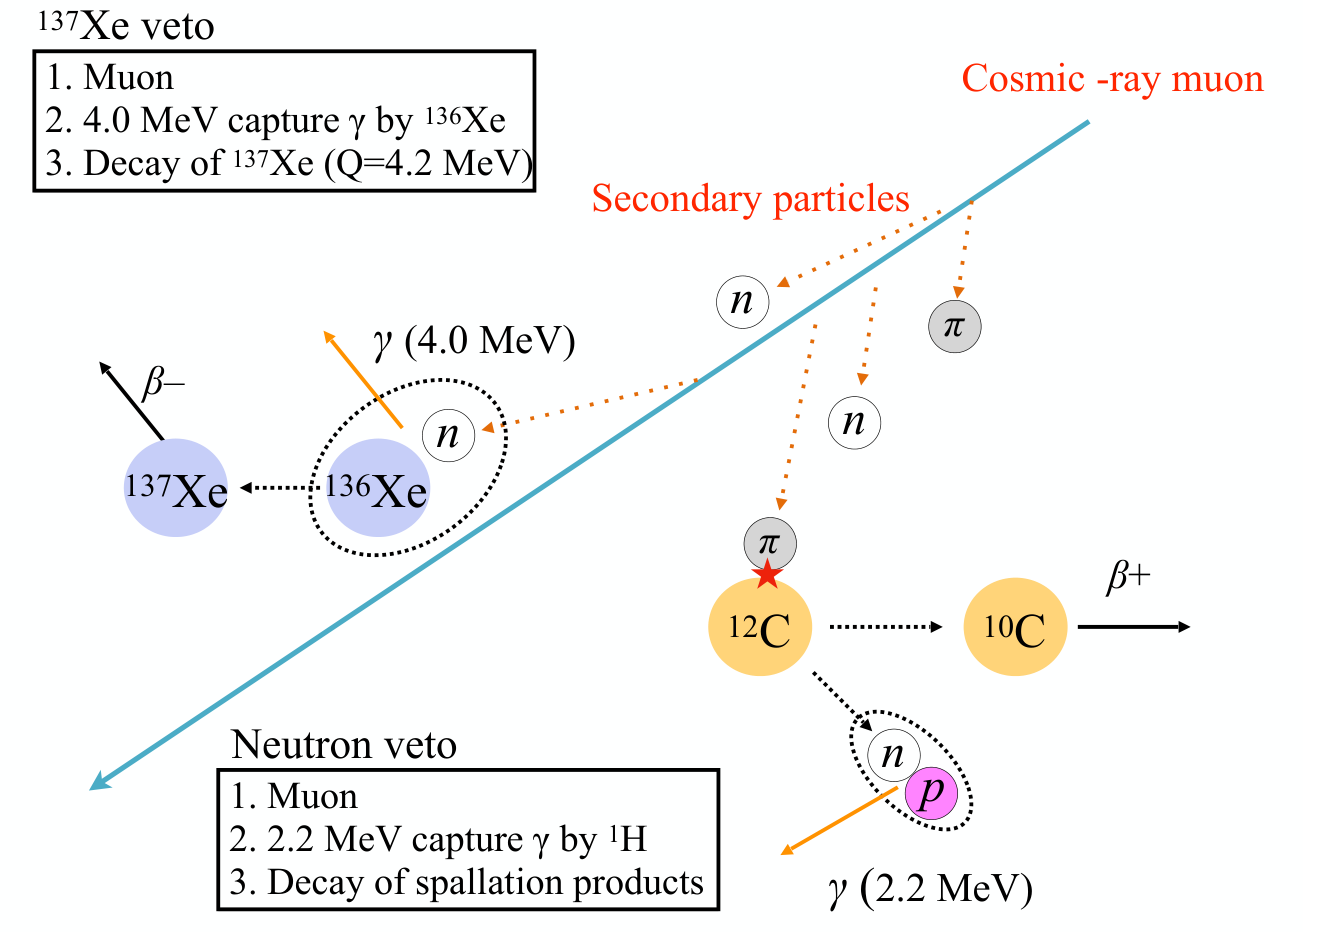
\includegraphics[scale=0.35]{spall_veto.png}
	\caption{A schematic of spallation veto with MoGURA neutrons}
	\label{fig:spall_veto}
\end{figure}

\subsection{Shower Veto}
As a cosmic-ray muon passes through the detector, it does not interact with uniform probability through its path. There is a point, where it deposits the most energy and spallates the most nuclei. Secondary decay products are correlated with this position. The shower veto identifies this location of high energy deposition and correlates background with this position.
\subsection*{PDF$(dE/dX,dL)$}
$dE/dX$, the distribution of energy deposition along muon tracks, and $dL$, the distance from the muon track to the candidate event, are correlated to the decay candidates. A two dimensional PDF$(dE/dX,dL)$ is constructed from muon data vy the following procedure:
\begin{enumerate}
	\item The cosmic ray muons are selected and their tracks reconstructed.
	\item The time when the muon enetered the ID $T_0$ is calculated.
	\item THe distance between the muon ID entrance and the generated point $L$ is calculated for each photon. Figure \ref{fig:showerphoton} shows the schematic of photon generation from cosmic muons. 
	\begin{equation}
		x^2_2=r^2+s^2_1-2x_1r\cos\theta
	\end{equation}
	\begin{equation}
		x_1+nx_2=c(t-t_0)
	\end{equation}
	Here, $n$ is the refractive index of the liquid scintillator. These equations are solved for $x_1$, the distance L can be obtained. For general analysis and reconstruction, only the PMT hit times of the first photons are used. However, for this calculation, multiple photons for each PMT are considered, referred to as multiTQ analysis. $L$ is calculated for each incident photon on each PMT. 
\end{enumerate}

\begin{figure}[htb]
	\centering
	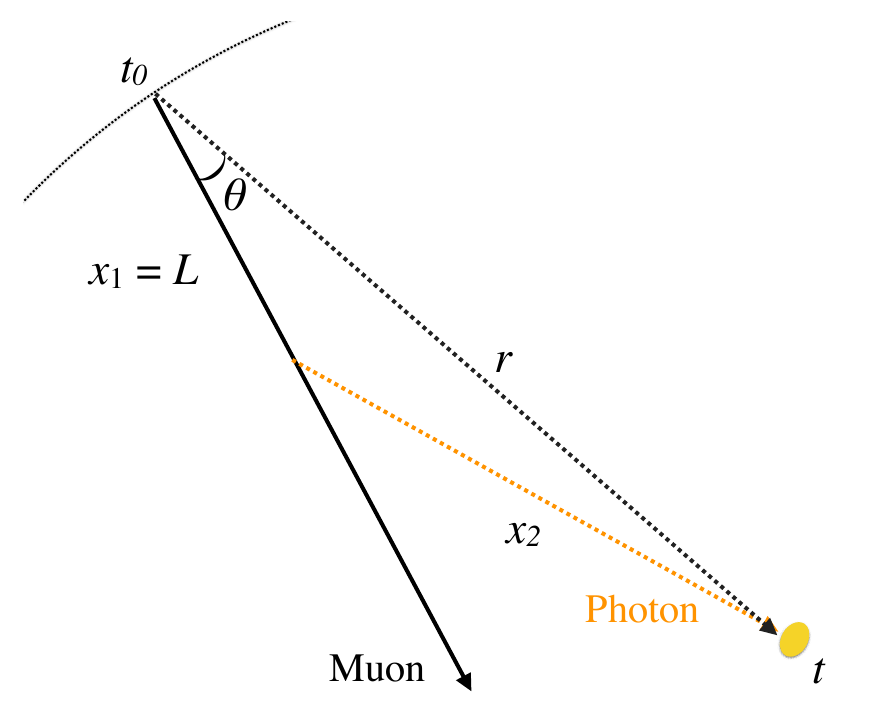
\includegraphics[scale=0.35]{showerphoton.png}
	\caption{$dE/dx$ reconstruction.}
	\label{fig:showerphoton}
\end{figure}

$^{12}$B is used for estimating the PDF$(dE/dX,dL)$ as it can be easily tagged by the $dT$ selection after muon events. Figure \ref{fig:shower_pdf} shows an example of a $dE/dX$ calculation result. The accidental event likelihood can also be calculated using the off-time events. The spalation backgrounds are rejected by calculting a likelihood ratio value of spallation vs accidental. THe log-likelihood ratio threshold used is -1.8, events with spallation-accidental logarithmic ratios below this value are classified as spallation backgrounds and rejected.

\begin{figure}[htb]
	\centering
	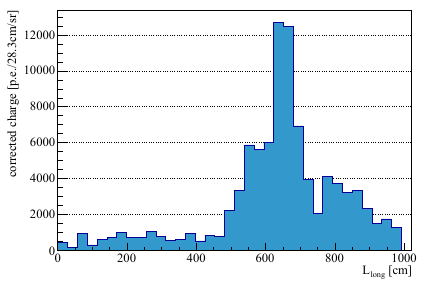
\includegraphics[scale=0.75]{shower_dedx.png}
	\caption{An example of a calculated $dE/dx$. The muon's largest energy deposit can be seen at $L_{long}=600$ cm.}
	\label{fig:shower_pdf}
\end{figure}

\subsection{Xenon Spallation Products}
The spallation products of Xenon are an important background to the \0nbb search. For the $2\nu\beta\beta^*$ search they obscure the endpoint of the \2nbb spectrum. Rejecting this background is important to both double-beta physics searches. However, these heavier nuclei can have half-lives of hours or longer, much longer than their Carbon-spallation counterparts, therefore, the MoGURA neutron veto is ineffective against these. 

For these backgrounds, a likelihood selection has been developed specifically for these "long-lived" spallation products. The method involves constructing PDFs of $dT$ (time since muon), $dR$ (spatial distance from the nearest neutron created by each muon), $ENN$ (Effective Number of Neutrons).

$^{136}$Xe spallation is characterized by the production of many free neutrons, these post-muon neutron captures are useful in identifying likely long-lived spallation isotopes. However, there is a high rate of accidental neutrons and unphysical detector noise that can be attributed to neutrons. The $ENN$, Effective Number of Neutrons, was developed to define a weighted counting of neutrons by who likely they are to be related to a given event. Each neutron following a muon is assigned a weight based on the spatial distributions of neutron captures from spallation products and accidentals. Figure \ref{fig:ENN_dR} shows the weight over $dR$.
\begin{equation}
	\label{eq:ENN}
	ENN = \sum_{neutrons}\frac{PDF_{spl.}(dR)}{PDF_{spl.}(dR)+PDF_{acc.}(dR)}
\end{equation}
The PDFs are the probability distributions of $dR$ which is the spatial distance between a candidate event and a neutron event. Spallation products and neutrons that originate from the same muon have a spatial correlation. The PDFs are shown in Figure \ref{fig:spall_dR}. $PDF_{spl.}(dR)$ is modeled with an exponentially modified Gaussian distribution, while $PDF_{acc.}(dR)$ is simply quadratic, assuming uniform distribution in space of uncorrelated events. The exponentially modified Gaussian function features 3 free parameters:
\begin{equation}
	f(x;\mu,\sigma,\lambda)=\frac{\lambda}{2}exp\left(\frac{\lambda}{2}(\mu+\lambda\sigma^2-2x)\right)erfc\left(\frac{\mu+\lambda\sigma^2-x}{\sqrt{2}\sigma}\right)
\end{equation}

$erfc(x)$ is the complementary error function defined as $erfc(x)=1-erf(x)$. The free parameters are determined using $^{10}$C data. The sum in equation \ref{eq:ENN} is over all the neutrons in a short window after a muon, it is a quantity assigned to each muon.

\begin{figure}[htbp]
	\centering
	\subcaptionbox{dR distribution for neutrons associated with spallation products and accidental neutrons\label{fig:spall_dR}}[0.45\textwidth]{
		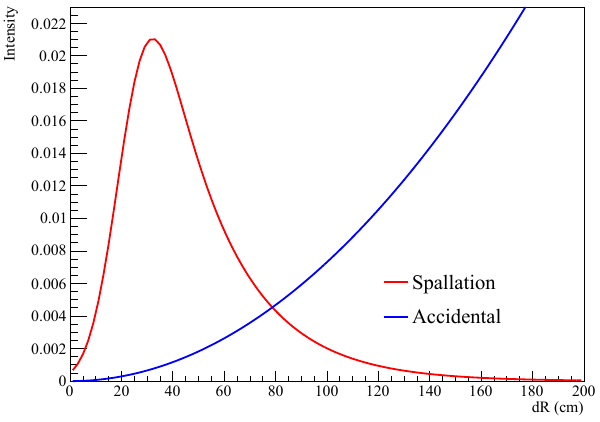
\includegraphics[width=0.45\textwidth]{spall_dR.png}}
	\hfill
	\subcaptionbox{Long-lived events\label{fig:longlived}}[0.45\textwidth]{
		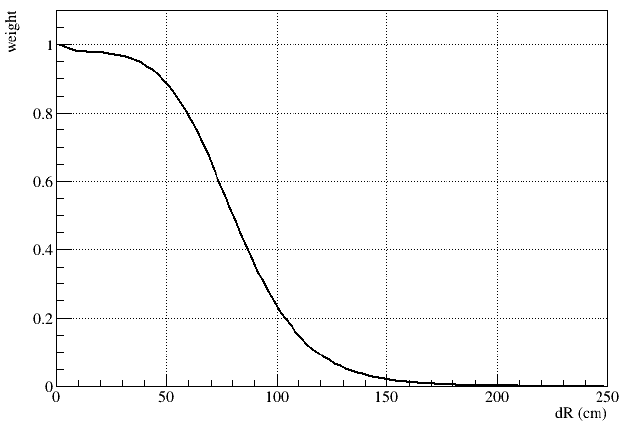
\includegraphics[width=0.45\textwidth]{ENN_dR.png}}
	\caption{Weighting factor function for ENN.}
	\label{fig:ENN_dR}
\end{figure}

\subsection*{Long-Lived Spallation Likelihood}
Long-lived spallation backgrounds are handled not by rejecting out of the analysis outright, but by separating long-lived spallation candidates into a separate spectrum to be fitted alongside the residual events. The long-lived data (LD) and the singles data (SD) are separated by calculating a likelihood ratio threshold. The likelihood ratio is defined as:
\begin{equation}
	R_L=\frac{L_{spl.}}{L(acc.)+L(spl.)}
\end{equation}
where $L_{acc}$ and $L_{spl}$ are the likelihood functions of accidental events and long-lived spallation backgrounds.

The spallation product likelihood is constructed from:
\begin{equation}
	L_{spl.}(dR_{near}, ENN, dT)=\sum_{spl. products}PDF(dT)\times PDF(dR_{near}, ENN)
\end{equation}
where the sum is calculated for all spallation isotopes listed in Table \ref{tab:spallproducts}. There is an implicit assumption that the time-component of the likelihood and the $PDF(dR, ENN)$ are independent. $L_{acc}$ is assumed to be uniform in time and is defined as:
\begin{equation}
	L_{acc.}(dR, ENN, dT) = PDF(dR, ENN)
\end{equation}

The likelihoods are constructed from FLUKA simulations and real muon data in KamLAND-ZEN. The long-lived likelihood uses FLUKA simulations of spallation product production and neutron ejection. The accidental likelihood uses events that occur after muons to get a data-informed $dR$ and $ENN$ distribution. Figure \ref{fig:likelihood_dR_ENN} shows the 2D profiles of the two likelihood functions. The differences are clear, in particular that the spallation products are more likely to have higher $ENN$ and lower $dR$. In order to avoid dividing by a joint 0 likelihood in the likelihood ratio, bin-smoothing is done to both likelihoods to extend them into the full range.

\begin{figure}[htbp]
	\centering
	\subcaptionbox{Spallation Products\label{fig:spall_dR_ENN}}[0.45\textwidth]{
		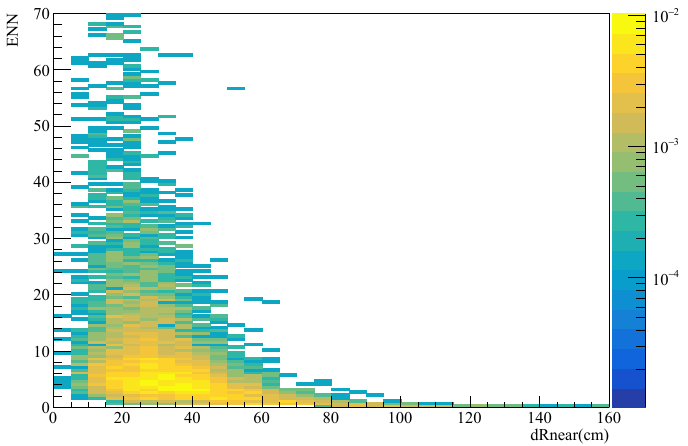
\includegraphics[width=0.45\textwidth]{spall_dR_ENN.png}}
	\hfill
	\subcaptionbox{Accidental events\label{fig:acc_dR_ENN}}[0.45\textwidth]{
		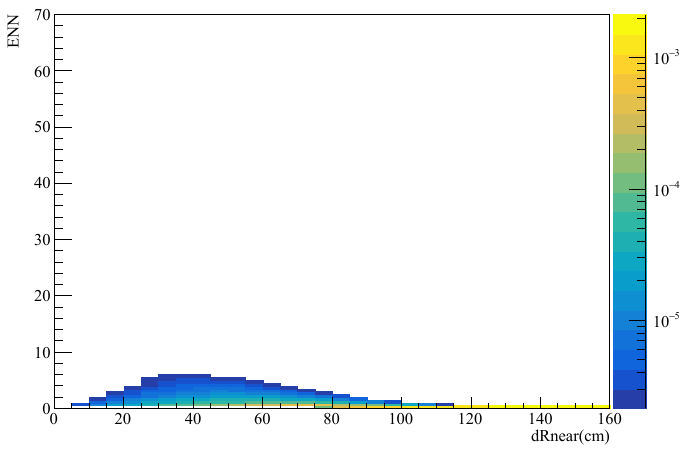
\includegraphics[width=0.45\textwidth]{acc_dR_ENN.png}}
	\caption{Weighting factor function for ENN.}
	\label{fig:likelihood_dR_ENN}
\end{figure}

Figure \ref{fig:LHR} shows the distributions of log-likelihood ratios, calculated from our PDFs from toy-MC trials. $10^6$ events are generated for each PDF. The log-likelihood ratio is $\log_{10}\left(1-\frac{L_{acc}}{L_{acc}+L_{spl}}\right)$, the logarithm is taken to bring all events into a similar range. With this definition, a smaller likelihood ratio or LHR means a higher likelihood of being a long-lived spallation product and a larger LHR indicates a higher likelihood of being an accidental event.
\begin{figure}[htb]
	\centering
	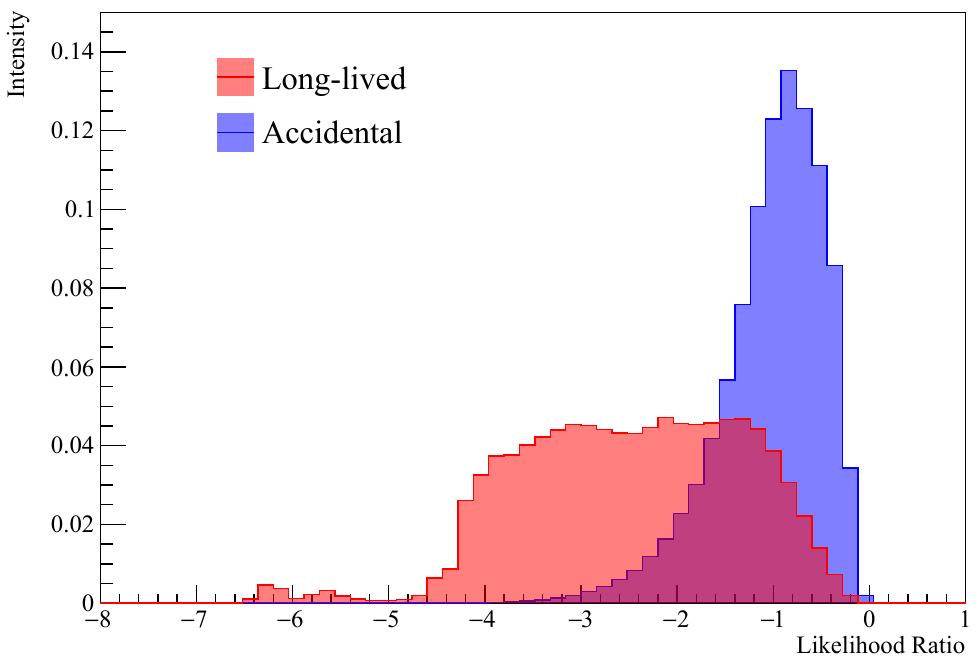
\includegraphics[scale=0.35]{LHR.png}
	\caption{Log-Likelihood ratio distributions generated from the PDFs by a ToyMC study. A clear separation between the distributions can be seen.}
	\label{fig:LHR}
\end{figure}

\subsection*{Figure of Merit}
To separate the data events into SD/LD datasets a threshold on the LHR variable must be determined. This threshold is determined by a Figure of Merit calculation (FOM).
\begin{equation}
	\text{FOM}=\frac{S(t)}{\sqrt{s(t)+B(t)}}
\end{equation}
$S(t)$ and $B(t)$ are the integrated LHR distributions above threshold, $t$, of signal and background generated by the toyMC study above. Due to inconsistent run conditions, including MoGURA livetime and efficiency, the datasets is separated into 3 time periods and a threshold is independently determined for each time period.
\begin{figure}[htb]
	\centering
	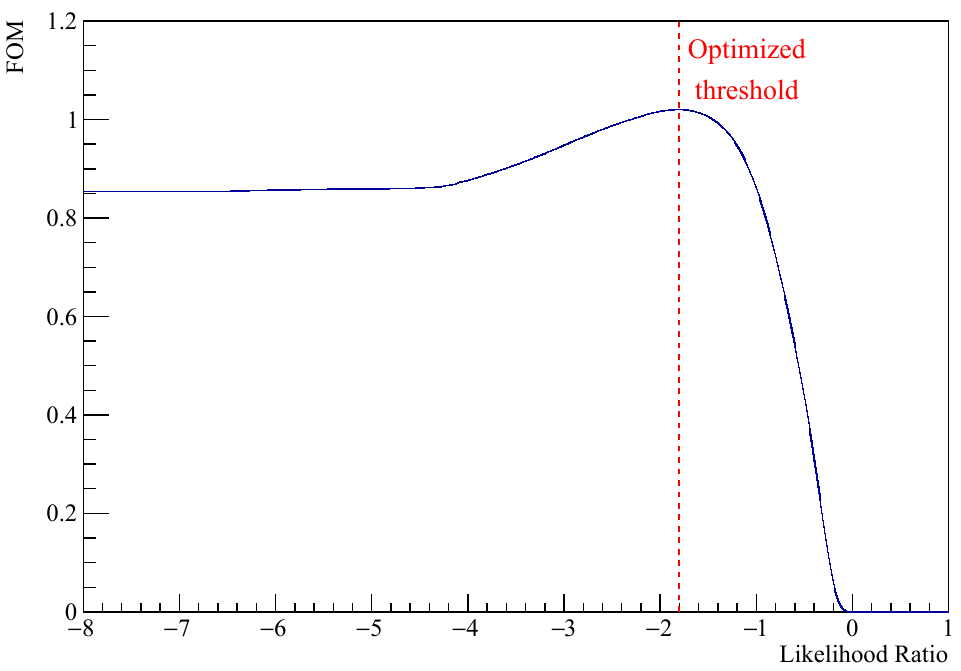
\includegraphics[scale=0.35]{FOM.png}
	\caption{Long-lived spallation veto Figure of Merit}
	\label{fig:FOM}
\end{figure}

\subsection*{Veto Efficiency}
\subsection*{Uncertainties}
\subsection*{Spectrum Distortion}

\subsection{Signal Inefficiency}
The effect of all these background vetoes on the \0nbb signal needs to be understood. This signal inefficiency is determined by calculating the livetime of the analysis. 

The livetime calculation is done by applying the same event selections to toy MC events distributed uniformly in time and space. Real detector data is used for the Muon-neutron pairs, delayed coincidence analysis, 1PPS trigger event, and missing waveform events. Livetime is the fraction of runtime leftover after event selection.
\begin{equation}
	\text{Livetime} = \frac{\text{\# of Toy MC events after event selection}}{\text{\# of generated Toy MC events}}\times \text{Runtime}
\end{equation}
The \2nbb$^*$ spectral fit is performed over long-lived spallation enriched and depleted events simultaneously. A later section describes this selection. For proper relative normalization, the livetime is calculated for both long-lived enriched and depleted samples. The deadtime of the KLZ physics analysis is listed in Table \ref{tab:deadtime}.
\begin{table}[htbp]
\centering
\caption{Summary of the deadtime}
\label{tab:deadtime}
\begin{tabular}{|l|c|}
\hline
\textbf{Event selection} & \textbf{Deadtime ratio [\%]} \\ \hline
Spallation veto & 14.64 \\ \hline
MoGURA neutron veto & 4.91 \\ \hline
$^{8}$Xe veto & 1.33 \\ \hline
Shower veto & 7.37 \\ \hline
$^{12}$B veto & 3.11 \\ \hline
Xe spallation veto & 8.56 \\ \hline
\begin{tabular}[c]{@{}l@{}}Detector deadtime veto\\(post PPS, after muons and missing waveforms)\end{tabular} & 9.47 \\ \hline
Hardware related & 0.0078 \\ \hline
Delayed coincidence Ra veto & 0.0013 \\ \hline
Delayed coincidence Reactor veto & 0.0010 \\ \hline
\textbf{Total} & \textbf{29.52} \\ \hline
\end{tabular}
\end{table}

The signal inefficiency of the double-pulse fitter and vertex Badness are omitted from table \ref{tab:deadtime}. This is due to the Toy MC livetime study not being done at the PMT hit level. Sections \ref{sec:dpfit} \& \ref{sec:badqualityevents} show that the signal inefficiency from these selections are negligible.

\chapter{Detector Calibration and MC Tuning}
\label{chapter:calibartion}
\thispagestyle{myheadings}
\graphicspath{{4_Chapter_Calibration/Figures/}}

Accurate modeling of physics events and detector response are essential for correct interpretations of KamLAND-ZEN experimental data. This chapter outlines the detector calibration and Monte-Carlo (MC) tuning methods used. Since the commissioning of KamLAND-ZEN 800, no deployed laser or radioactive source calibration was done. This was to avoid any radioactive contamination from inserting these components into the detector. Thus, known backgrounds are the primary tools for detector calibration.
\cite{klz800_arxiv}

\section{Detector Calibration}
The KamLAND detector has taken data for over 20 years. The energy scale, nonlinearity, bias, resolution, and vertex bias and resolutions have been well calibrated and studied. However, it is important to understand the variation of the detector performance over time. Electronics issues, such as HV reduction, channel loss, and detector work can affect our reconstructions. 
\subsection{Variation of Energy Scale Over Time}
As PMT channels are lost or deteriotate into bad channels, or have their gains adjusted, the energy scale of the detector can vary over time. Variation from the beginning of the analysis period in 2019 and until the end of KLZ-800 data-taking in 2024, the energy scale varied by 3\%. 

\begin{figure}[htb]
    \centering
    % Left subplot (A) - Time variation
    \begin{subfigure}[b]{0.48\textwidth}
        \centering
        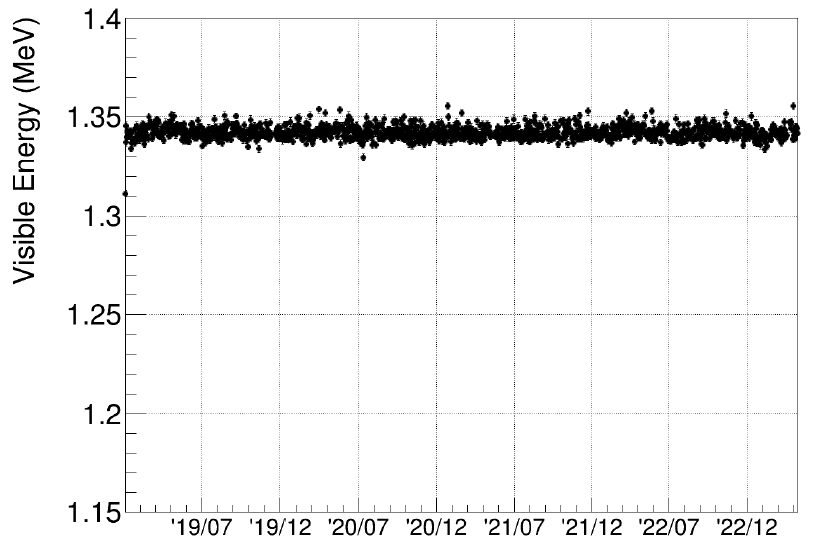
\includegraphics[width=\textwidth]{K40_PEEK_Time.png}
        \caption{Time variation}
        \label{fig:time_variation}
    \end{subfigure}
    \hfill
    % Right subplot (B) - Histogram
    \begin{subfigure}[b]{0.48\textwidth}
        \centering
        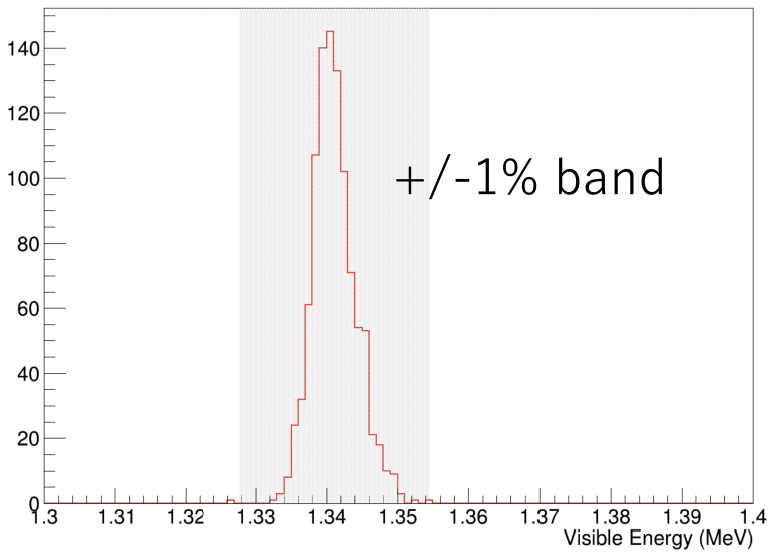
\includegraphics[width=\textwidth]{PEEK_energy.png}
        \caption{Histogram among runs (\%) axis}
        \label{fig:histogram}
    \end{subfigure}
    
    \caption{Time variation of $^{40}$K peak after correction. (A) Time variation of 
    energy scale is corrected using $^{40}$K and this figure is a check using $^{40}$K itself. 
    (B) Fluctuations among runs are within 1\% (gray band).}
    \label{fig:figure51}
\end{figure}
\subsubsection*{$^{40}$K PEEK Gammas}
Reconstructing the $^{40}$K-$\gamma$ peak from balloon PEEK material can help calibrate the energy scale over time. The PEEK material is located 550cm above the center of the detector and is a consistent source of $^{40}$K radioactive decays. The decay energy of the $^{40}$K electron-capture decay to $^{40}$Ar has an energy of $Q_{EC}=1504$ keV. However, as the energy scale of the detector decreases as you move from the center of the detector. This EC-$\gamma$ peak is observed at around $E_{vis}=1.35$ MeV in KamLAND-ZEN. These $^{40}$K PEEK events are selected by the following simple selection:
\begin{itemize}
	\item Passes Flasher Veto
	\item Passes Muon Veto
	\item Passes 2msec veto after muons
	\item cylindrical volume selection around PEEK material ($450<z<600$,$\rho<250$ cm)
\end{itemize}

\subsubsection*{Neutron Capture Gammas}
The KamLAND energy scale is primarily set by neutron captures on Hydrogen. Figure \ref{fig:neutron_capture_energy} shows the variation in neutron capture visible energy over time in XeLS and KamLS. Events are taken simply in a time window following muons. Due to post-muon instability, such as high after-pulsing, PMT ringing, and baseline shifts, the time directly after muons is excluded. An on-off time analysis is performed to subtract any incidental backgrounds and resolve the neutron capture energy distribution.
\begin{itemize}
    \item On-time window : $400<dT<1500 \mu sec$
    \item Off-time window : $2800<dT<4000 \mu sec$
\end{itemize}
\begin{figure}[htb]
	\centering
	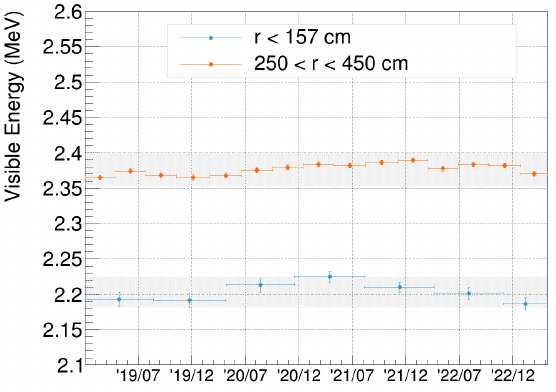
\includegraphics[scale=0.65]{neutron_escale.png}
	\caption{Neutron capture energy over KLZ-800 data-taking. The blue and orange points correspond to XeLS and KamLS respectively. Gray bands show $\pm1\%$ deviation from the average. Note that the energy scale is 7\% higher in KamLS due to the higher scintillator light-yield.}
	\label{fig:neutron_capture_energy}
\end{figure}
\subsubsection*{$2\nu\beta\beta$ Rate}
The tail of the \2nbb decay spectrum is another useful handle on variations in energy scale over time. In the abscence of any XeLS leakage out of the inner balloon, the rate of \2nbb events in an energy range can be used to verify the energy scale. We apply all the \0nbb analysis event selections and a further $1.85<E_{vis}<2.35$ MeV energy selection to select the \2nbb-dominant region. Figure \ref{fig:2nu_stability} shows minor fluctuations, but no clear trend upward or downwards.
\begin{figure}[htb]
	\centering
	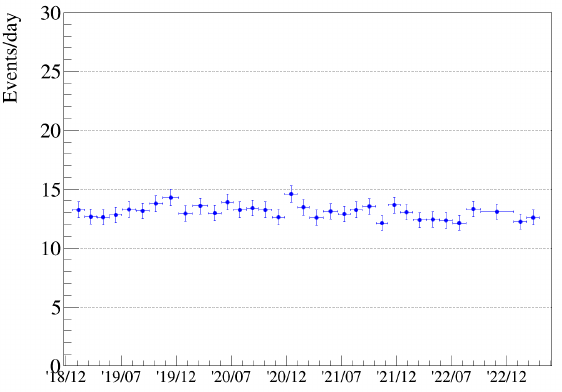
\includegraphics[scale=0.65]{2nu_trend.png}
	\caption{The event rate in the \2nbb dominant energy region over KLZ-800 data-taking.}
	\label{fig:2nu_stability}
\end{figure}
\subsection{MoGURA Stability}
Cosmic ray muon induced spallation reactions are a constant source of well understood background. MoGURA's dead-time-free electronics allow it to observe neutron capture's closer in time to the original muons. This higher tagging efficiency than KAMFEE provides more data that can be used for calibration.

The MoGURA stability performance over time is marked by the neutron capture rate and distributions. Figure \ref{fig:neutron_capture_energy} shows the variation over time of MoGURA's neutron tagging performance. The neutron selection in MoGURA was outline in section \ref{sec:mogura_neutron_reco}.
\begin{figure}[htb]
	\centering
	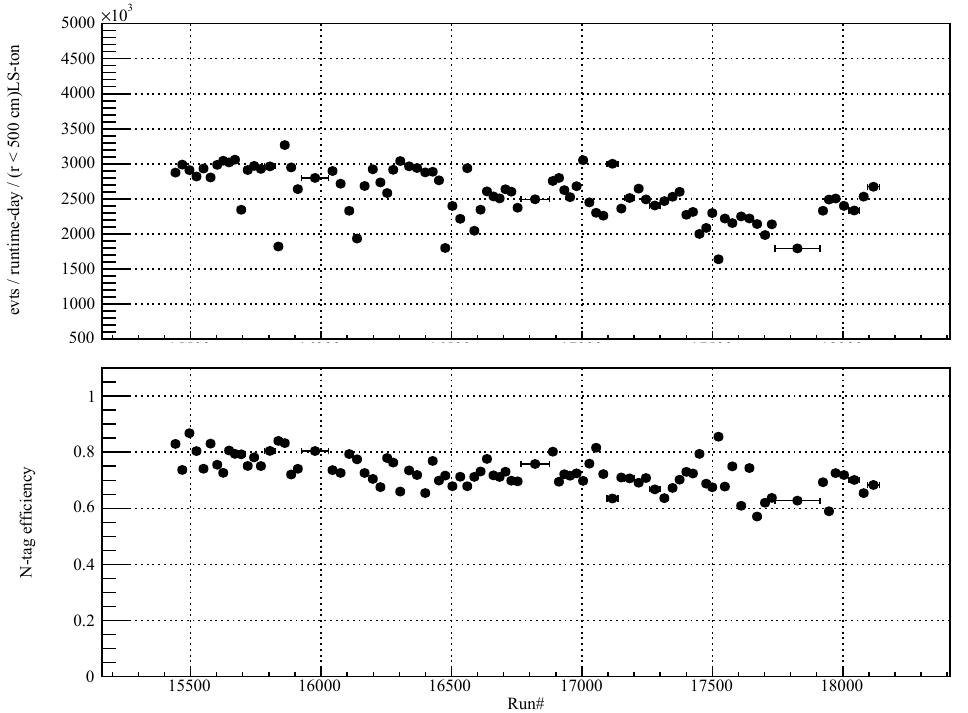
\includegraphics[scale=0.35]{neutron_capture_trend.png}
	\caption{MoGURA's neutron capture rate and neutron tagging efficiency over KLZ-800 data-taking.}
	\label{fig:neutron_capture_trend}
\end{figure}
\subsubsection*{$^{10}$C tagging Stability}
$^{10}$C is an easily isolated, well-understood background that can be further used to monitor detector stability. $^{10}$C tagging via triple coincidence was described in section \ref{sec:mogura_neutron_veto}. Note that for this study, the $^{10}$C selection was adjusted from the \0nbb analysis for higher signal purity.
\begin{itemize}
    \item Select events in KamLS volume $(250<r<400 cm)$ and veto the corrugateed tube $(r>250 cm\& z>0)$
    \item $2.0<E_{vis}<5.0 $ MeV
    \item On-time window: $10<dT<90$ sec
    \item Off-time window: $300<dT<1000$ sec
\end{itemize}
The on-time window begins at 10 seconds to exclude the $^{6}$He spallation background with a 1.16 second lifetime and $Q_\beta=3.5$ MeV. Figure \ref{fig:c10_mogura} shows the characteristic distributions that identify the dataset as $^{10}$C. The rate is estimated by fitting an exponential plus constant background to the $dT$ distribution. The $dR$, distance to nearest neutron, distribution is modeled by an $exGaussian$, exponentially modified Gaussian. The variation in $^{10}$C rate and mean of the exGaussian function are shown in Figure \ref{fig:C10_stability}
\begin{figure}[htb]
	\centering
	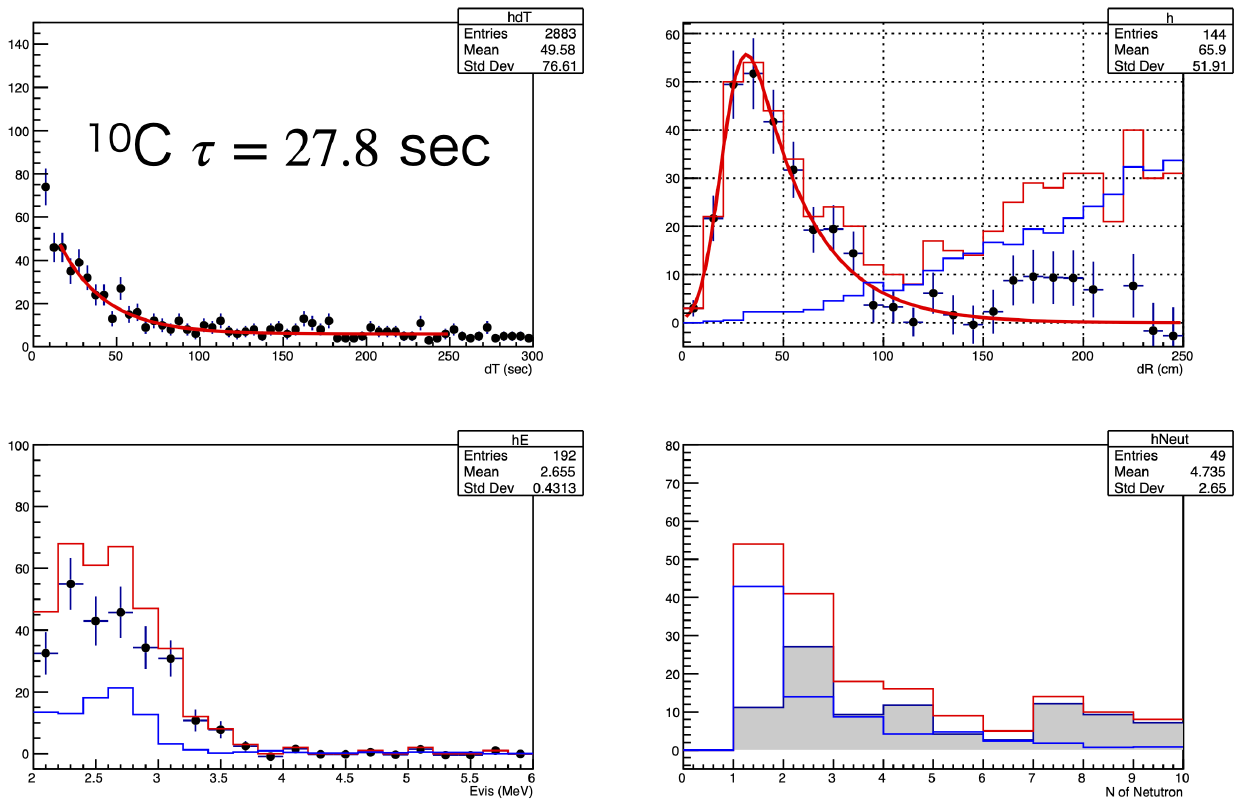
\includegraphics[scale=0.35]{mogura_c10.png}
	\caption{Characteristic distributions of $^{10}$C decays. Red and blue histograms show on-time and off-time events respectively, and the black markers or grey histograms show the subtracted distributions (on-time - off-time). }
	\label{fig:c10_mogura}
\end{figure}

\begin{figure}[htb]
    \centering
    \begin{subfigure}[b]{0.48\textwidth}
        \centering
        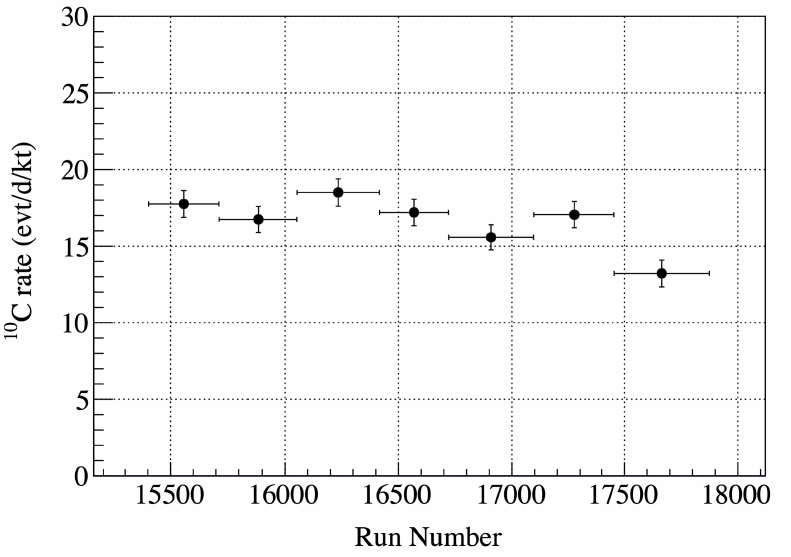
\includegraphics[width=\textwidth]{c10_rate.png}
    \end{subfigure}
    \hfill
    \begin{subfigure}[b]{0.48\textwidth}
        \centering
        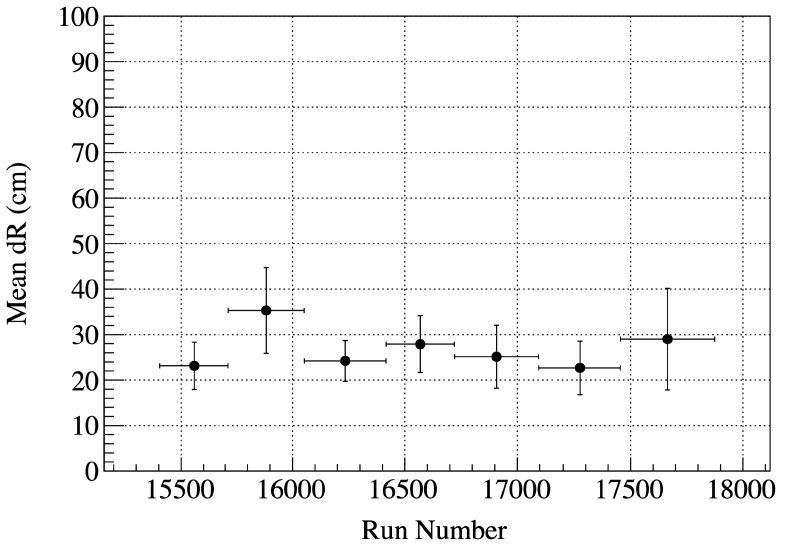
\includegraphics[width=\textwidth]{c10_dist.png}
    \end{subfigure}
    
    \caption{Time variation of $^{10}$C rate and dR distribution shape over KLZ-800 data-taking.}
    \label{fig:C10_stability}
\end{figure}

\section{MC Tuning}
KamLAND physics simulation is built on two simulation tools: GEANT4 and FLUKA. GEANT4 is used to simulate the distributions of signals, backgrounds decays, and scintillation light propagation in KamLAND detector media. KamLAND's GEANT4-based simulation tool chain is called KLG4Sim. FLUKA is used to simulate cosmic-ray muon induced spallation. Namely for neutron multiplicity and topology and spallation isotope production. 
\subsection{Geant4 (KLG4)}
KLG4 simulations used in this thesis analysis were tuned in \cite{ozaki_phd} and \cite{takeuchi_phd}. This section describes their prior work in tuning KLG4 parameters.
\subsubsection*{KamLS Tuning}
KamLS properties, the outer scintillator volume without dissolved xenon, are tuned using source calibration data taken on January 16, 2018. The calibartion deployment involved moving a composite radioactive soure between -550 and 550 cm in 50cm intervals. With 20 minutes of data-taking at each position. Table \ref{tab:calib_soure} describes the source composition.

\begin{table}[h]
\centering
\caption{Summary of radioactive source. Estimated intensities are as of January 17, 2018 on which the calibration DAQ was taken.}
\label{tab:calib_soure}
\begin{tabular}{lccc}
\hline
Construction date & \multicolumn{3}{c}{Aug. 24, 2015} \\
DAQ date & \multicolumn{3}{c}{Jan. 16, 2018} \\
Source ID & \multicolumn{3}{c}{Kam-41 (composite source)} \\
\hline
 & $^{137}$Cs & $^{68}$Ge & $^{60}$Co \\
Particle & 1$\gamma$ & 2$\gamma$ & 2$\gamma$ \\
Energy (keV) & 661.7 & 511.0 & 1173.2, 1332.5 \\
Initial Intensity (Bq) & 181 & 419 & 322 \\
Estimated Intensity (Bq) & 180 & 356 & 234 \\
\hline
\end{tabular}
\end{table}
Figure \ref{fig:calib_source} shows the $N_{hit}$ and total charge spectra of the composite source, with clearly visible gamma peaks. The gamma peaks are used to calibrate the nonlinearity of KamLS energy scale. The figure also shows the tuned KLG4 spectra that agrees well with data after tuning.

The energy scale is also tracked through position, via calibration source deployment. The deployment data was used to tune material properties like attenuation length, re-emission probabilities, and scattering probabilities. Figure \ref{fig:calib_source_pos} shows the position dependence of total charge for each source isotope. The variability and simulation reproducibility with tuning is deteriorates as we move from the center of the detector. The physics analysis presented in this thesis focuses on data within 250cm. In this region, the deviation is within 2\%.
\begin{figure}[htb]
    \centering
    \begin{subfigure}[b]{0.48\textwidth}
        \centering
        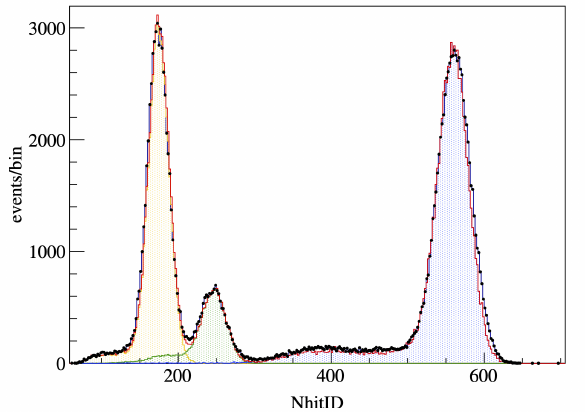
\includegraphics[width=\textwidth]{calib_source_nhit.png}
    \end{subfigure}
    \hfill
    \begin{subfigure}[b]{0.48\textwidth}
        \centering
        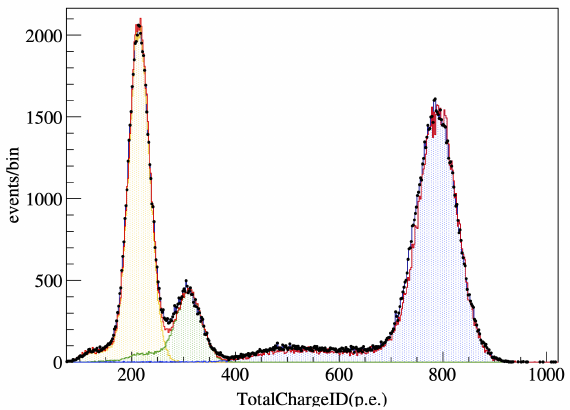
\includegraphics[width=\textwidth]{calib_source_charge.png}
    \end{subfigure}
    
    \caption{$N_{hit}$ and total charge distribution of source calibration. Black plots show data and colored histograms (orange: 137 Cs, green: 68Ge, blue: 60 Co) show MC simulation. MC spectra are well tuned to data in both $N_{hit}$ and total charge. Figures from \cite{ozaki_phd}}
    \label{fig:calib_source}
\end{figure}

\begin{figure}[htb]
	\centering
	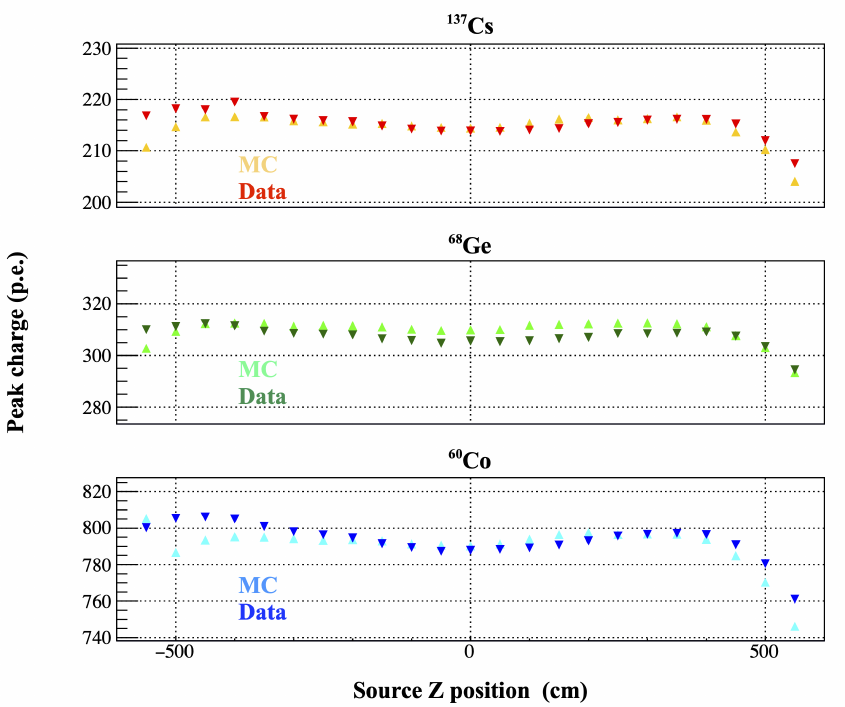
\includegraphics[scale=0.35]{calib_source_pos.png}
	\caption{Position dependence of total charge peak for each calibration source isotope \cite{ozaki_phd}}
	\label{fig:calib_source_pos}
\end{figure}

\subsubsection*{XeLS Tuning}
There are no source calibration located in XeLS. Alternatively, some background sources are available to calibrate the detector. $^{222}$Rn is mixed in XeLS by emanation from pipeline or buffer tanks during xenon resolving work. A sequential decay of daughter isotopes $^{214}$Bi-Po can be tagged using delayed coincidence and they exists only in XeLS. The half life of $^{222}$Rn is 3.8 days and after completion of xenon resolving work, $^{222}$Rn does not supplied. Thus $^{214}$Bi-Po as high statistic calibration source is available only in first several months of KamLAND-Zen 800 observation. Birk's constant, attenuation length, scattering probability, LS time properties, and re-emission for XeLS are tuned using $^{214}$Bi-Po.

\subsubsection*{Position-dependent Energy Correction}

Position dependence, over radius and $\theta$, of visible energy in XeLS is observed using the $^{214}$Po $alpha$ decay peak. The deviation from the center of the detector is reproduced in KLG4 as shown in Figure \ref{fig:po214_alpha}. The MC correction factors were tuned to ensure that the MC \0nbb decay peak in XeLS does not have a position dependence.

\begin{figure}[htb]
\centering
\begin{subfigure}[b]{0.45\textwidth}
    \centering
    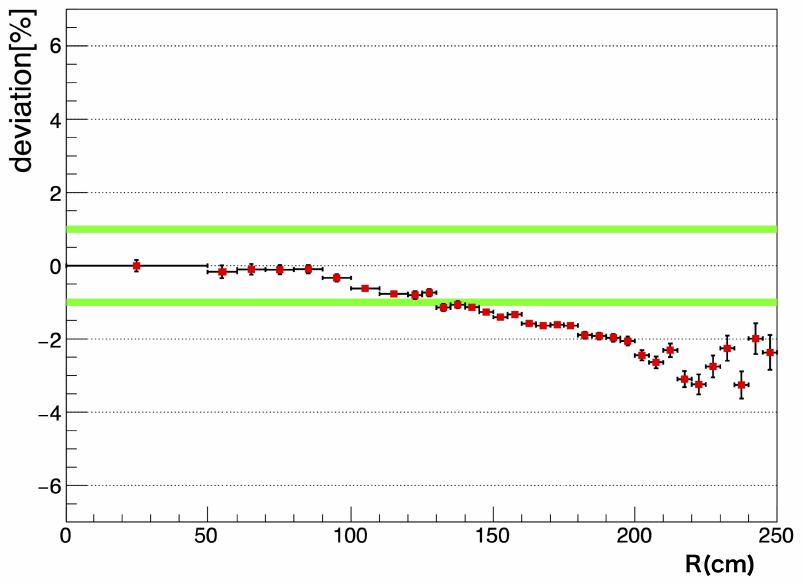
\includegraphics[width=\textwidth]{po214_data.png}
    \caption{Data}
    \label{fig:po214_data}
\end{subfigure}
\hfill
\begin{subfigure}[b]{0.45\textwidth}
    \centering
    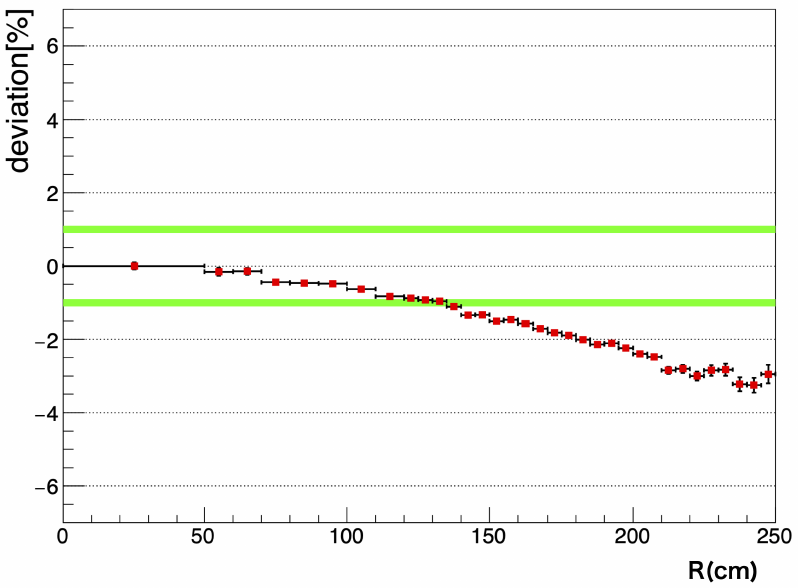
\includegraphics[width=\textwidth]{po214_mc.png}
    \caption{MC (before correction)}
    \label{fig:po214_mc_before}
\end{subfigure}

\vspace{1cm}

\begin{subfigure}[b]{0.45\textwidth}
    \centering
    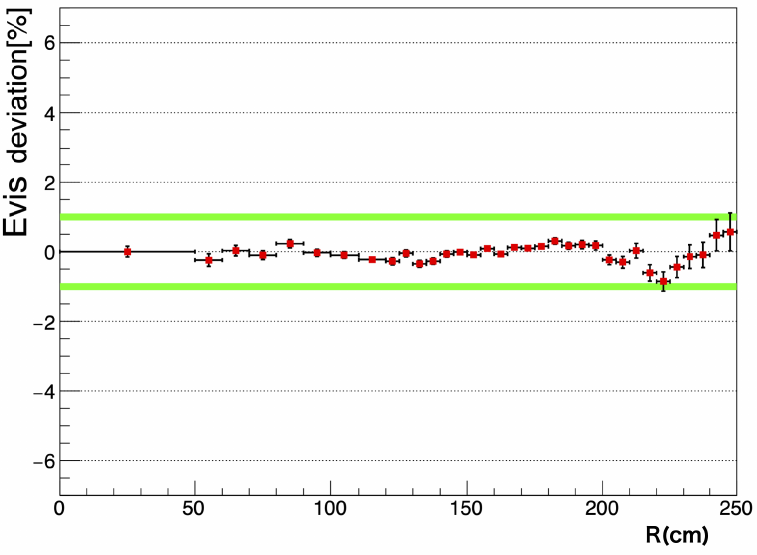
\includegraphics[width=\textwidth]{po214_mc_corr.png}
    \caption{MC (after correction)}
    \label{fig:po214_mc_after}
\end{subfigure}

\caption{Radius dependence of total charge of $^{214}$Po. Figures from \cite{ozaki_phd}.}
\label{fig:po214_alpha}
\end{figure}

\subsubsection*{Energy Non-Linearity}
The visible energy and the energy deposited by charged particles have a nonlinear relation due to the scintillation quenching and the contribution of Cherenkov light. The following model is well known as Birks formula:
\begin{equation}
    \label{eq:birks_law}
    \frac{dL}{dx}\propto\frac{dE/dx}{1+kB\cdot dE/dx^\prime}
\end{equation}
where $dL/dx$ is light yield per unit length along particle track, $dE/dx$ is energy deposited per unit length, and $kB$ is the Birks' constant which is material dependent. Charged particles also emit cherenkov light, the proportion of the light yield attributed to cherenkov radiation is denoted by the chrenkov-scintillation ratio, $R$. Tagged $^{214}$Bi data is used to tune $kB$ and $R$. The tagged $^{214}$Bi data in XeLS is primarily from the early $^{222}$Rn-rich period. The tuning analysis was performed in \cite{ozaki_phd} and \cite{takeuchi_phd}. Figure \ref{fig:kb_r_chisquare} shows a $\Delta\chi^2$ scan over $kB$ and $R$ and the best fit of $(kB, R)=(0.31, 0.01)$. These are the values used in KLG4 for background and signal simulation. Figure \ref{fig:bipo_tune} shows the result of XeLS tuning. The BiPo decay energies are matched to data and the spatial correlation between the coincident decays agree.

\begin{figure}[htb]
	\centering
	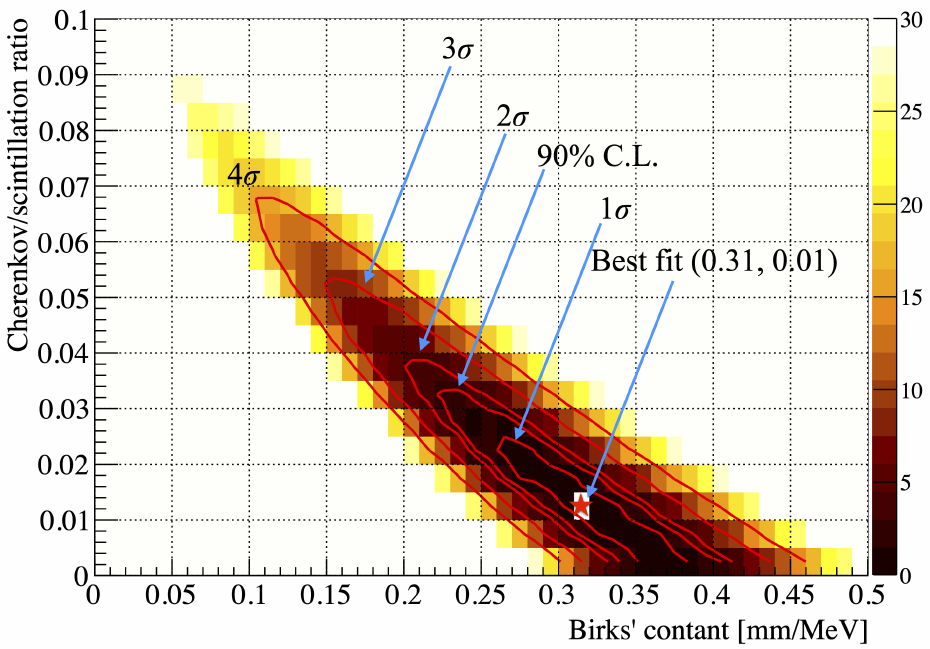
\includegraphics[scale=0.35]{kb_r_chisquare.png}
	\caption{$\Delta\chi^2$ scan over $kB$ and $R$}
	\label{fig:kb_r_chisquare}
\end{figure}

\begin{figure}[htb]
    \centering
    \begin{subfigure}[b]{0.48\textwidth}
        \centering
        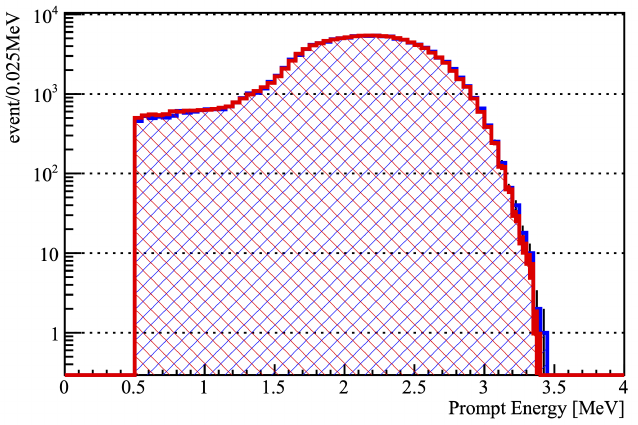
\includegraphics[width=\textwidth]{bi214_spec_tune.png}
    \end{subfigure}
    \hfill
    \begin{subfigure}[b]{0.48\textwidth}
        \centering
        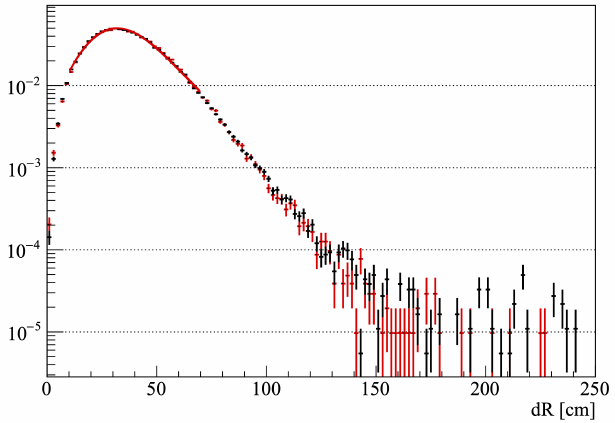
\includegraphics[width=\textwidth]{bipo_dR.png}
    \end{subfigure}
    
    \caption{Tuned $^{214}$Bi-$\beta$ decay energy spectrum and spatial correlation of delayed-coincidence Bi-Po decays. Figures from \cite{takeuchi_phd}}
    \label{fig:bipo_tune}
\end{figure}
\subsubsection*{Energy Scale}
The overall energy scale of KamLS and XeLS are tuned by the neutron capture gamma peak of 2.2 MeV. XeLS introduces extra quenching by the xenon which reduces the light yield in XeLS slightly. Figure \ref{fig:neutron_capture_energy} shows the peak energies used. This is the same dataset used for the energy scale time variation check.
\subsection{FLUKA}
FLUKA simulation software is used to predict cosmic muon spallation isotope yields and neutron production. The FLUKA version used in this modeling is FLUKA 2011.08.patch. Simulations and the results are described in \cite{klz_xenon_spallation}. Studies and measurements performed in KamLS are outlined in \cite{kamland_spallation_2009}.
\subsubsection*{Simulation Configuration}
The FLUKA physics process packages used in these spallation studies are listed in Table \ref{tab:fluka_process}. FLUKA is only used  to generate the production of spallation isotopes and neutrons, their decays and isomer production are disabled. The subsequent decays and neutron capture gammas are simulated in GEANT4. 

Cosmic ray muon spallation is simulated by injecting muons into a cylindrical XeLS volume of 10 m radius and 40 m height. The inner balloon radius is only ~2m. The volume within 10 m from the side and 5m from the exit is excluded from the analysis to avoid boundary effect. The MUSIC package is used to generate the cosmic ray muon energy distribution\cite{MUSIC}. MUSIC takes in the detailed geometric description of the Kamioka mine where KamLAND is located. The generated energy distribution is fed into FLUKA and fired into the simulation's XeLS volume. The mean simulated muon energy is $260\pm1$ GeV. The simulation yields a neutron capture time of $\tau=207.0\pm0.3\mu$sec which is consistent with the previously measured value. The muon charge ratio is taken to be $\mu^+/\mu^-=1.3$ in this simulation\cite{kamei_phd}.

\begin{table}[h]
\centering
\caption{FLUKA physics processes. From Ref.\cite{klz_xenon_spallation}.}
\label{tab:fluka_process}
\begin{tabular}{lll}
\hline
card & Physics & Status \\
\hline
DEFAULTS & A set of physics models & PRECISIO(n) \\
PHOTONNUC(lear) & Gamma interactions with nuclei & Activated \\
MUPHOTON & Muon photonuclear interaction & Activated \\
PHYSICS & Emission of light fragments & Activated by COALESCE(nse) \\
PHYSICS & Emission of heavy fragments & Activated by EVAPORAT(ion) \\
PHYSICS & Ion electromagnetic dissociation & Activated by EM-DISSO(ciation) \\
PHYSICS & Decay and isomer production & Activated by RADDECAY \\
\hline
\end{tabular}
\end{table}

\subsubsection*{Radioactive Decays}
As previously described, FLUKA is used only for the direct spallation isotope production and neutron captures. The subsequent radioactive decays are simulated in the "Radioactive Decay" package in Geant4. The GEANT4 version used is Geant4.10.6.p01 with G4ENSDFSTATE2.2 for the Evaluated Nuclear Structure Data File (ENSDF) \cite{ENSDF}. Table \ref{tab:xenon_spallation_products} lists the xenon spallation produts considered in this study. In total, 32 isotopes are selected that have production rates exceeding 0.01/day/XeLS-kton in the Region of Interest (ROI). Figure \ref{fig:xenon_spallation_spectrum} shows the simulated energy spectra. 

\begin{figure}[htb]
	\centering
	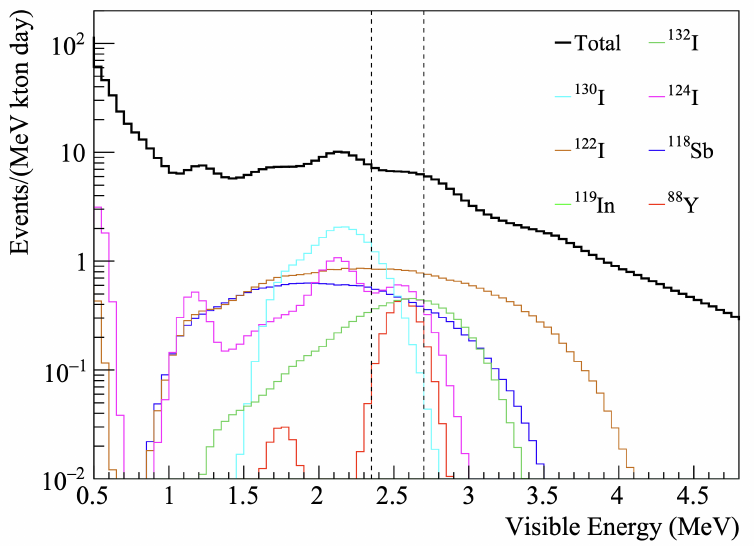
\includegraphics[scale=0.35]{xenon_spallation_spectra.png}
	\caption{Simulated energy spectra of $^{136}$Xe spallation products including their decay chain.}
	\label{fig:xenon_spallation_spectra}
\end{figure}

\begin{table}[ht]
\centering
\caption{Breakdown of $^{136}$Xe spallation products. Isotopes with production rates exceeding 0.01 /day/XeLS-kton in the Region of Interest (ROI) were considered and included in the background model.}
\label{tab:xenon_spallation_products}
\begin{tabular}{lllccc}
\hline
isotope & decay mode & Q-value & half-life & ROI & Total \\
 & & (MeV) & (s) & (day-kton)$^{-1}$ & (day-kton)$^{-1}$ \\
\hline
$^{88}$Y & EC/$\beta^+$/$\gamma$ & 3.62 & $9.212 \times 10^6$ & 0.110 & 0.136 \\
$^{90m}$Zr & IT & 2.31 & $8.092 \times 10^{-1}$ & 0.012 & 0.093 \\
$^{90}$Y & EC/$\beta^+$/$\gamma$ & 6.11 & $9.212 \times 10^5$ & 0.024 & 0.095 \\
$^{96}$Tc & EC/$\beta^+$/$\gamma$ & 2.97 & $3.698 \times 10^5$ & 0.012 & 0.059 \\
$^{98}$Rh & EC/$\beta^+$/$\gamma$ & 5.06 & $5.232 \times 10^2$ & 0.011 & 0.076 \\
$^{98}$Rh & EC/$\beta^+$/$\gamma$ & 3.63 & $7.488 \times 10^4$ & 0.088 & 0.234 \\
$^{103}$Ag & EC/$\beta^+$/$\gamma$ & 4.28 & $4.152 \times 10^3$ & 0.012 & 0.160 \\
$^{104m}$Ag & EC/$\beta^+$/$\gamma$ & 4.28 & $2.010 \times 10^3$ & 0.018 & 0.111 \\
$^{107}$Cd & EC/$\beta^+$/$\gamma$ & 3.43 & $1.944 \times 10^3$ & 0.019 & 0.135 \\
$^{108}$In & EC/$\beta^+$/$\gamma$ & 5.16 & $3.480 \times 10^3$ & 0.089 & 0.194 \\
$^{110}$In & EC/$\beta^+$/$\gamma$ & 3.89 & $1.771 \times 10^4$ & 0.053 & 0.236 \\
$^{110m}$In & EC/$\beta^+$/$\gamma$ & 3.89 & $4.146 \times 10^3$ & 0.066 & 0.351 \\
$^{110}$Sn & EC/$\beta^+$/$\gamma$ & 3.85 & $1.080 \times 10^3$ & 0.027 & 0.122 \\
$^{113}$Sb & EC/$\beta^+$/$\gamma$ & 3.92 & $4.002 \times 10^2$ & 0.036 & 0.231 \\
$^{114}$Sb & EC/$\beta^+$/$\gamma$ & 5.88 & $2.094 \times 10^2$ & 0.020 & 0.297 \\
$^{115}$Sb & EC/$\beta^+$/$\gamma$ & 3.03 & $1.926 \times 10^3$ & 0.031 & 0.839 \\
$^{116}$Sb & EC/$\beta^+$/$\gamma$ & 4.71 & $9.480 \times 10^2$ & 0.071 & 0.939 \\
$^{118}$Sb & EC/$\beta^+$/$\gamma$ & 3.66 & $2.160 \times 10^2$ & 0.165 & 1.288 \\
$^{116}$Te & EC/$\beta^+$/$\gamma$ & 2.90 & $5.201 \times 10^6$ & 0.016 & 0.054 \\
$^{115}$Te & EC/$\beta^+$/$\gamma$ & 4.64 & $3.489 \times 10^2$ & 0.012 & 0.124 \\
$^{117}$Te & EC/$\beta^+$/$\gamma$ & 3.54 & $3.720 \times 10^3$ & 0.052 & 0.584 \\
$^{119}$I & EC/$\beta^+$/$\gamma$ & 3.51 & $1.146 \times 10^3$ & 0.053 & 0.533 \\
$^{120}$I & EC/$\beta^+$/$\gamma$ & 5.62 & $4.896 \times 10^3$ & 0.091 & 0.953 \\
$^{122}$I & EC/$\beta^+$/$\gamma$ & 4.23 & $2.178 \times 10^2$ & 0.289 & 1.965 \\
$^{124}$I & EC/$\beta^+$/$\gamma$ & 3.16 & $3.608 \times 10^5$ & 0.190 & 1.654 \\
$^{108}$I & $\beta^-$/$\gamma$ & 2.95 & $4.450 \times 10^4$ & 0.195 & 1.188 \\
$^{132}$I & $\beta^-$/$\gamma$ & 3.58 & $8.262 \times 10^3$ & 0.148 & 0.427 \\
$^{134}$I & $\beta^-$/$\gamma$ & 4.18 & $3.150 \times 10^3$ & 0.043 & 0.183 \\
$^{121}$Xe & EC/$\beta^+$/$\gamma$ & 3.75 & $2.406 \times 10^3$ & 0.100 & 0.540 \\
$^{125}$Cs & EC/$\beta^+$/$\gamma$ & 3.09 & $2.802 \times 10^3$ & 0.012 & 0.266 \\
$^{126}$Cs & EC/$\beta^+$/$\gamma$ & 4.82 & $9.840 \times 10^1$ & 0.011 & 0.080 \\
$^{128}$Cs & EC/$\beta^+$/$\gamma$ & 3.93 & $2.196 \times 10^2$ & 0.031 & 0.229 \\
\hline
\end{tabular}
\end{table}

\subsubsection*{Tuning With $^{10}$C}
FLUKA simulations of radioactive decays and neutron capture gamma do not include detector effects and reconstruction performance. The information given by the FLUKA simulation includes the capture points of neutron captures but not the reconstructed vertices. 

To approximate the effect of event reconstruction, the true neutron capture positions from FLUKA are convolved with a Gaussian resolution distribution. The neutron detection efficiency is also emperically modeled by:
\begin{equation}
    \epsilon(\log_10Q_\mu)=\epsilon\left(1-\frac{1}{1+e^{-\sigma(\log_10Q_\mu-a)}}+b\right)
\end{equation}
The neutron detection efficiency is known to be particularly sensitive to baseline fluctuations in the immediate aftermath of a muon. Since, the baseline recovery time depends on the muon charge, the neutron detection efficiency, $\epsilon$, is assumed ot depend on the charge.

$(1+e^{-\sigma x})^{-1}$ is a sigmoid function which mimics the error function and $Q_{\mu}$ is muon charge. $\sigma$ controls the steepness of the sigmoid function's transition. Free parameters, $\sigma, a, b$ are tuned to reproduce the $dR$ and $ENN$ distributions of $^{10}$C as shown in Figure \ref{fig:fluka_tuning}. $dR$ is the spatial distance to the nearest neutron of a given shower, while $ENN$ is the "effective number of neutrons". Vertex resolution affect both of these variables, while the neutron tagging efficiency primarily affects $ENN$.
\begin{figure}[htb]
        \centering
    \begin{subfigure}[b]{0.48\textwidth}
        \centering
        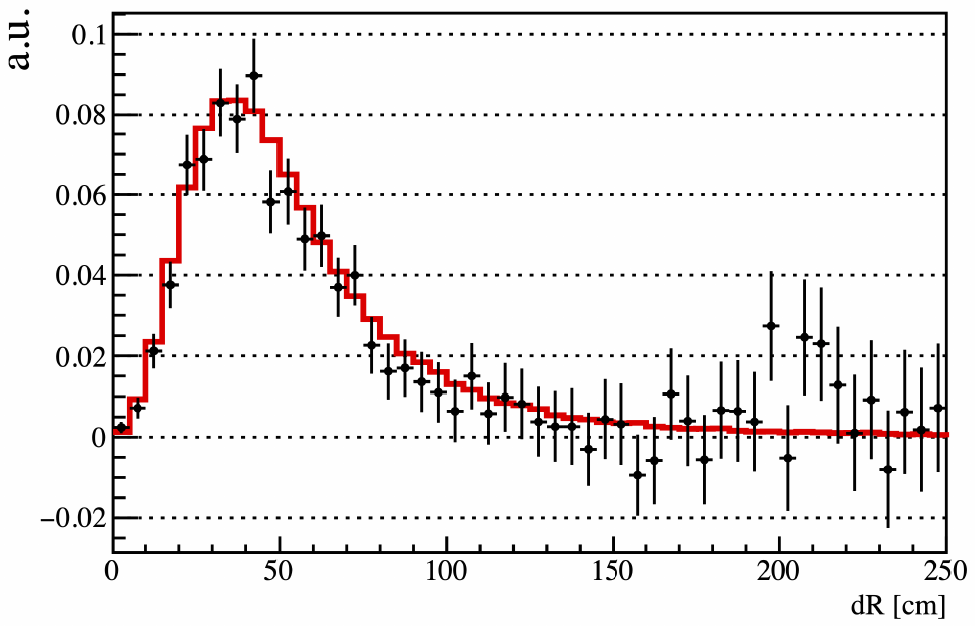
\includegraphics[width=\textwidth]{c10_tune_dR.png}
    \end{subfigure}
    \hfill
    \begin{subfigure}[b]{0.48\textwidth}
        \centering
        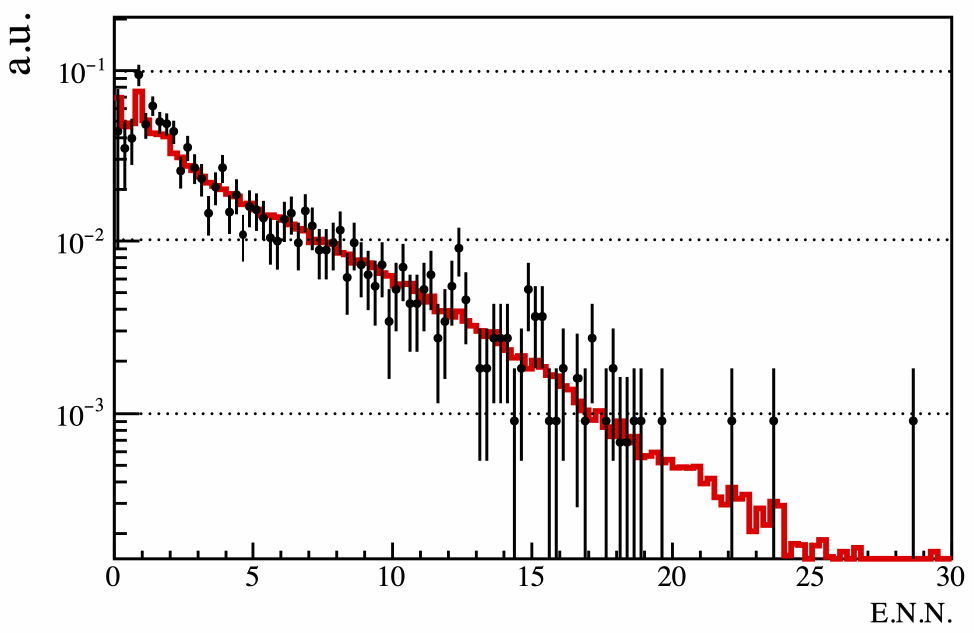
\includegraphics[width=\textwidth]{c10_tune_ENN.png}
    \end{subfigure}
    
    \caption{Tuned $^{10}$C $dR$ (left) and $ENN$ (right) distributions from FLUKA (red curve) and data (black dots) Figures from \cite{miyake_phd}}
    \label{fig:fluka_tuning}
\end{figure}

%==========================================================================%
% Bibliography
\newpage
\singlespace
\bibliographystyle{plain}

% each subdirectory can have its own BiBTeX file
\bibliography{thesis} % same bib file as main thesis
\cleardoublepage

%==========================================================================%
% Curriculum Vitae
% \phantomsection\addcontentsline{toc}{chapter}{Curriculum Vitae}

\begin{center}
    {\LARGE \bf CURRICULUM VITAE}\\[0.5in]
    {\large \bf Hasung Song}\\[0.1in]
    Department of Physics\\
    Boston University\\
    Email: hwsong@bu.edu\\
    % Add more contact info as needed
\end{center}

\vspace{0.3in}

\section*{Education}
\begin{itemize}[leftmargin=*]
    \item \textbf{Ph.D. in Physics}, Boston University, 2019--Present
    \item \textbf{M.Sc. in Physics}, Boston University, 2019--2022
    \item \textbf{B.Sc. in Physics}, University of California, Berkeley, 2016-2018
\end{itemize}

\section*{Professional Experience}
\begin{itemize}[leftmargin=*]
    \item \textbf{Post-Baccalaureate Researcher}, University of California, Berkeley, 2018--2019
\end{itemize}

\section*{Selected Publications}
\begin{itemize}[leftmargin=*]
	\item "Search for Majorana Neutrinos with the Complete KamLAND-Zen Dataset" KamLAND-Zen Collaboration,	arXiv:2406.11438 [hep-ex] (2024)
	\item "Eos: conceptual design for a demonstrator of hybrid optical detector technology" T. Anderson et al. JINST 18 P02009 (2023)
	\item "KamNet: An integrated spatiotemporal deep neural network for rare event searches in KamLAND-Zen" A. Li, et al. Phys. Rev. C 107, 014323 (2023)
	\item "RFSoC-based front-end electronics for pulse detection" S.N. Axani et al. 2024 JINST 19 P03013 (2024)
	\item "Search for the Majorana Nature of Neutrinos in the Inverted Mass Ordering Region with KamLAND-Zen" KamLAND-Zen Collaboration, Phys. Rev. Lett. 130, 051801 (2023)
\end{itemize}

\section*{Scientific Collaborations}
\begin{itemize}[leftmargin=*]
	\item EoS Collaboration 2023--Present
	\item NuDOT Collaboration 2022--Present
    \item KamLAND Collaboration 2020--Present
    \item NIM+ 2020--2021
	\item Mu2E Collaboration 2018--2019
\end{itemize}

\section*{Conferences and Presentations}
\begin{itemize}[leftmargin=*]
    \item "Getting Excited About Double Beta Decay in KamLAND-Zen", APS DNP, Talk, Boston, MA, 2024.
    \item "Understanding KamNet Performance in KamLAND-ZEN with ML Interpretability", SLAC Summer Institute, Poster, SLAC, 2023.
    \item "KamLAND-Zen's New ML Tricks", Neutrino Physics and Machine Learning, Talk, Northeastern University, 2023.
    \item "Rejecting Spallation Backgrounds in KamLAND-ZEN with KamNet", Neutrino, Poster, Seoul, Korea, 2022.
    \item "Rejecting Spallation Backgrounds in KamLAND-ZEN with KamNet", TAUP, Poster, Valenica, Spain, 2021.
    \item "Neutrinoless Muon-to-Positron Conversion at Mu2e", APS April Meeting, Talk, Denver, Colorado, 2019.
\end{itemize}

\section*{Teaching Experience}
\begin{itemize}[leftmargin=*]
    \item Physics 211 General Physics I, Teaching Assistant, Boston University, Summer 2020.
    \item Physics 211 General Physics I, Teaching Assistant, Boston University, Fall 2019.
\end{itemize}

\section*{Professional Service}
\begin{itemize}[leftmargin=*]
    \item Member, Graduate Student Council, Boston University Physics Department, 2019--Present.
\end{itemize}

\end{document}
 

%==========================================================================%
\end{document}
